% ------------------------------------------------------------------------------
% Mathematics Project Report Template
% by Jon Shiach 2019
% Manchester Metropolitan University
% ------------------------------------------------------------------------------
\documentclass[11pt]{report} 

\usepackage{projectreport}

% Define 'keyword' environment if not using elsarticle
\newenvironment{keyword}{\par\noindent\textbf{Keywords:} }{\par}


% ------------------------------------------------------------------------------
% Enter your details here
% ------------------------------------------------------------------------------
\newcommand{\name}{Celumusa H Zulu}
\newcommand{\degree}{Master of Commerce}
\newcommand{\programme}{Information Technology Management}
\newcommand{\projecttitle}{The role of IT leadership in realising the return on investment of AI coding assistants.}
\newcommand{\supervisor}{Dr. Siyabonga Mhlongo}
\newcommand{\submissionyear}{2026}

% ------------------------------------------------------------------------------
% Document
% ------------------------------------------------------------------------------
\begin{document}

\maketitle

% ------------------------------------------------------------------------------
% Top matter
% ------------------------------------------------------------------------------
\chapter*{Abstract}
\addcontentsline{toc}{chapter}{Abstract}
The rapid adoption of generative artificial intelligence (AI) coding assistants is changing how software engineering teams develop, test, document, and deliver software. Despite previous research showing that AI coding assistants can be effective at improving developer productivity, it does not follow that such improvements will result in better ROI. The benefits of integrating AI in a company also depend on how well it manages, promotes and integrates the technology in the routine software development process. This study investigates how organisational culture and strategic leadership influence the realisation of ROI from AI coding assistants in software engineering teams. The study is guided by Technology Value Realisation Framework \autocite{Kuna2014} as well as the Socio-Technical Systems perspective, which provide a basis for understanding how technological benefits depend on both organisational and human factors.

This research employs the quantitative research design to explore the linkages among various factors like organisational culture, strategic leadership, AI coding assistant assimilation quality, and the return on investments. The study focuses on software engineering teams of medium-scale and large organisations in South Africa that have implemented the AI coding assistant technologies. Data was collected through a well-structured survey with the help of the Likert scale. The return on investment in case of AI coding assistants has been examined on three levels, which are the impact at the level of task, the impacts regarding integration and coordination at the level of workflow, and the effects on the financial and futuristic aspect of the company. AI coding assistants assimilation quality is considered to be the mediating variable along with organisational readiness, the maturity and experience of the team, and length of the adoption as the control variables.

The study aims to fill the gap in existing body of knowledge by examining opportunities to realise return on investment from the usage of AI programming assistants and the impact of organisation-related issues on the overall productivity of programmers. The research will use statistical approaches, like, Structural Equation Modeling, to establish the reliability and validity of the measurement model as well as test the relationships between variables in the study. The research is expected to determine if organisational culture and strategic leadership directly impact AI-related ROI and contribute to the proper assimilation of AI coding assistants into software engineering processes. 

The study contributes to AI value realisation research by linking technology performance to organisational culture and leadership. The study results will provide practical tips for software engineering managers and companies aiming to deploy AI coding assistants in the way that would guarantee positive productivity and business results.

\begin{keyword}
 Artificial intelligence, AI coding assistants, organisational culture, strategic leadership, technology value realisation, assimilation quality, return on investment, software engineering.
\end{keyword}

\chapter*{Declaration}
\addcontentsline{toc}{chapter}{Declaration}
I, {\name}, certify that the dissertation submitted by me for the {\degree} in {\programme} degree at the University of Johannesburg is my independent work and has not been submitted by me for a degree at another university.

\vspace{2cm}
------------------------------------------ \newline
{\textsc \name} \newline
(No signature required)

\chapter*{Dedication}
\addcontentsline{toc}{chapter}{Dedication}
To my Mother, who always believe in me,	my kids and to all my Siblings who always believe in me. \newline To Evelyn Manosa thank you for your support to make this study possible.

\chapter*{Acknowledgements}
\addcontentsline{toc}{chapter}{Acknowledgements}
First and foremost, infinite gratitude and appreciation to my Creator, Who has given me the
will to start studying again and the endurance to see this through in a time when my world was
turned on its head. My perseverance, accomplishments and very being are only by Your will.

Also, sincerest gratitude to my Kids, who had to endure my absence whilst completing this study. You are the very foundation my success is built on.

My deepest gratitude to my Mother, my Sister and my brother’s as well for always remembering
me in your prayers.

My sincerest appreciation to my Supervisor Dr. Siyabonga Mhlongo, who has always been my
light through this journey. You got me started on this, thank you for seeing me through to the
finish line.

I’d also like to extend my sincerest appreciation to all the people that took their precious time
and completed the survey to make this study possible.

\phantomsection
\tableofcontents
\markboth{Contents}{}
\clearpage

\phantomsection
\addcontentsline{toc}{chapter}{List of Acronyms} %
\printglossary[title=List of Acronyms,type=\acronymtype,style=long,nonumberlist,toctitle=List of Acronyms]
\markboth{List of Acronyms}{}
\clearpage

\phantomsection
\addcontentsline{toc}{chapter}{List of Figures} %
\listoffigures
\clearpage

% ------------------------------------------------------------------------------
% Main matter
% Chapters are added to the document using the \include{chapterx} command
% ------------------------------------------------------------------------------
\newpage
\setcounter{page}{0}
\pagenumbering{arabic}
\glsresetall

% ------------------------------------------------------------------------------
% Chapter 1
% ------------------------------------------------------------------------------
\chapter{Introduction} % enter the name of the chapter here
\label{cha:ch1_introduction} % enter the chapter label here (for cross referencing)

\section{Introduction} 
\label{sec:Introduction} 
This chapter introduces the study and also provides the background for examining the role of IT leadership in achieving ROI from AI coding assistants. It outlines the research problem being addressed and discusses the significance of the topic. Furthermore the chapter also presents the research questions and objections of this study. The final section of this chapter will provide an overview of the research methodology and theoretical framework used to guide the study.

\section{Background and context} 
\label{sec:Background and context} 
Artificial intelligence (AI) is one of the structural factors that has a significant impact on productivity and competitive advantages \autocite{Gillespie2025}. As of 2023, generative AI systems have developed from being an experiment to reaching the phase of implementation within organizational processes \autocite{Gillespie2025}. Recent reports from around the world show that organizations allocate more money to AI since they expect clear monetary outcomes, cost savings, and improved performance of organizational processes \autocite{Gillespie2025}. Research on information systems and management has transcended from the stage of adoption to the understanding of added value meanings with the emphasis on differentiation of organizational value created from investments in AI systems as a function of organizational governance and management performance, not technology excellence \autocite{Hossain2025}. 

In software engineering, the use of generative AI tools are among the most noticeable forms of AI-enabled augmentation \autocite{Peng2023}. Providing developers with functionalities such as code suggestions and entire code functions in real time based on context, documentation, and debugging \autocite{Peng2023}.Practical controlled experiments provide conclusive evidence that AI-assisted developers complete software development tasks faster and report increased productivity of about 55.8\% compared with control groups \autocite{Peng2023}. Collaboration between humans and AI systems is a paradigm shift from the traditional concept of automation, in which AI enhances developers’ capabilities rather than replacing them with machines \autocite{Peng2023}. Initial performance improvements demonstrated in controlled promising experiments may not necessarily guarantee long-term organizational performance benefits. Empirical studies report considerable variation in the productivity gains from AI-assisted software development tasks across software development teams and organizations. 

As it has been long noted, organization culture and management style have been generally believed to affect the implementation success of new technologies. Within the digital sphere, values and practices will drive the culture of experimentation, learning, and data use in decision making as well as a positive attitude to tech adoption. New findings reveal that digital culture explains the linkage between human AI skills and innovation outcomes, and that culture readiness mediates the performance impact of AI Investments \autocite{An2024}. Similarly, this applied also to employees' engagement in AI, ethical AI management or leadership impacts toward strategic alignment. Even though the significance of digital culture and leadership is being gradually recognized by most researchers, current research findings on AI Adoption is more fragmented \autocite{An2024}. A significant number of recent works investigated AI adoption under the macro-organizational view or focused on the impacts for personal performance only instead of integrating digital culture, management and ROI in the software industry \autocite{Peng2023}.

Generative AI (GenAI) has been increasingly adopted by african companies to address resource constraints and operational inefficiencies. Similarly, there is evidence that developing nations have tried extensively with AI and have positive views about AI’s capabilities to boost productivity at work \autocite{Gillespie2025}. Yet, literature to date highlights difficulties around digital skills pipelines, governance maturity and leadership capability among others in adopting GenAI technologies \autocite{Hughes2026}. In this context, organisational culture and leadership remain particularly critical. If these factors are not supported by a clear strategic vision, trust and a learning orientation, AI adoption is likely to be less about value creation and more about segmentation or symbolism. The digital transformation landscape in Africa is a valid environment for exploring the impact of socio-organizational factors on the achievement of returns from AI technologies.



\section{Rationale of the study} 
\label{sec:Rationale of the study} 

\section{Problem statement} 
\label{sec:Problem statement} 

\section{Significance of the study} 
\label{sec:Significance of the study} 

\section{Overview of the theoretical/conceptual framework} 
\label{sec:Overview of the theoretical/conceptual framework} 

\section{Research aim and objectives} 
\label{sec:Research aim and objectives} 

\section{Research questions} 
\label{sec:Research questions} 

\section{Scope and delimitation} 
\label{sec:Scope and delimitation} 

\section{Methodology overview} 
\label{sec:Methodology overview} 

\section{Ethical considerations} 
\label{sec:Ethical considerations} 

\section{Dissertation structure} 
\label{sec:Dissertation structure} 

\section{Chapter summary} 
\label{sec:Chapter summary} 
% ------------------------------------------------------------------------------
% Chapter 2
% ------------------------------------------------------------------------------
\chapter{Literature Review} % enter the name of the chapter here
\label{cha:ch2_literature} % enter the chapter label here (for cross referencing)

% ------------------------------------------------------------------------------
% Introduction
% ------------------------------------------------------------------------------
\section{Introduction}
\label{sec:Introduction}
Generative AI has become one of the most used technologies in different fields to perform various tasks where high levels of knowledge and information are required. This is different from traditional AI in the sense that this technology emphasizes cognitive complexity within the output created and responding to the need for community-specific interpretation, refinement, and integration. In software development, artificial intelligence is used in the form of coding-monitoring assistant tools that are included in the software-development environment to facilitate code generation, fixing bugs in the software, and creating documentation.

Empirical studies on the impact of generative AI on human productivity and output quality revealed that, under conditions of structured task design, a significant increase in human output is achieved. In a large-scale experimental design, the availability of generative AI tools resulted in a reduction on task completion time and an increase in output quality. The results achieved were statistically significant for the total sample, while the results were more pronounced for low-performing individuals \autocite{Noy2023}. The results support the view that generative AI tools can produce productivity gains at the individual task level.

However, the productivity gains at the task level do not necessarily translate into organizational return on investment. Research on AI investment at the firm level indicates that the performance effects are heterogeneous and conditional. AI investment is linked with growth through innovation and product development channels; however, the level and stability of the returns depend on the capabilities of the organization \autocite{Babina2024}. The market reaction to AI investment announcements is mixed, indicating the level of awareness among investors about the risk and capabilities \autocite{Lui2021}.

These studies all circle back to the same basic idea: AI capability does not produce value; rather, value is produced when the technological tools are embedded in the organizational systems. More recent studies have suggested another component: a digital organizational culture can influence the innovation outcome of AI capability \autocite{An2024}. Leadership can also play a part in influencing the development of trust and embedding AI usage \autocite{Schneider2023}.

Despite the recent increase in research on the performance effects of AI, little research has appeared that combines the effects of organizational culture and leadership into a structured ROI model for AI coding assistants in software development teams. This chapter synthesizes global empirical research on AI productivity and firm performance, critically evaluates the impact of organizational conditions, and focuses the research question more specifically on the South African market, where empirical ROI research has yet to be conducted.


% ------------------------------------------------------------------------------
% Chapter 3
% ------------------------------------------------------------------------------
\chapter{Research Methodology} % enter the name of the chapter here
\label{cha:ch3_methodology} % enter the chapter label here (for cross referencing)

\section{Introduction}
\label{sec:Introduction}
This chapter presents and justifies the methodological approach adopted to examine the influence of organisational culture and leadership on the return on investment (ROI) realised from AI coding assistants in software engineering teams. Given the complexity of the constructs under investigation, organisational culture, leadership, the assimilation quality of AI coding assistants, and ROI, it was essential that the research design be methodologically sound, so as to support the validity and generalisability of the findings. \textcite{Creswell2018} argues that the research design adopted should align closely with the research question(s) and the underlying theoretical framework. As this study sought to test relationships between constructs, to assess a mediating effect, and to do so while accounting for the measurement structure of each construct, a quantitative design combining preliminary correlational analysis with partial least squares structural equation modelling (PLS-SEM) was adopted. The chapter proceeds by outlining the research philosophy, research design, research hypotheses, population and sampling strategy, measurement and operationalisation of constructs, data collection procedure, data analysis techniques, research limitations, and the ethical considerations that guided the research.

\section{Research Philosophy}
\label{sec:Research Philosophy}
This paper is based on a post-positivist epistemology, which posits that social phenomena can be studied in a systematic manner, although measurement can never be perfect \autocite{Creswell2018}.

\subsection{Suitability of Post-Positivism for This Study}
\label{sec:Suitability of Post-Positivism for This Study}
The hypothesis testing process measures to what extent the relationships described in the conceptual framework are valid based on data. In quantitative analysis, hypotheses originate from theoretical frameworks presented in literature and are compared with empirical information. Consequently, researchers can determine whether or not links exist between different factors including organisational culture, leadership, the introduction of artificial intelligence, and profitability. Hypothesis testing is one of the key processes in quantitative investigations because it enables examining the above-mentioned theoretical frameworks and identifying whether or not the data support the proposed dependent and independent variables \autocite{Creswell2018}.

\begin{itemize}
	\item \textbf{Testing hypothesised relationships}
\end{itemize}
When testing relationships between concepts, one must verify the relationships indicated in the conceptual scheme against empirical data. In quantitative research, hypotheses are usually derived from the structure theories provided by literature. Thus, in quantitative studies, the researcher can state whether any relationships exist between such variables as organisational culture, leadership style, AI adoption, or ROI, etc. Hypothesis testing in quantitative research is of utmost importance since it allows testing theoretical schemes \autocite{Creswell2018}.

\begin{itemize}
	\item \textbf{Measuring latent variables}
\end{itemize}
Latent constructs are abstract concepts that cannot be measured directly, although they can be assessed through multiple indicators. In this study, organisational culture, leadership, and the assimilation quality of AI coding assistants were treated as latent constructs, as each represents complex organisational behaviour rather than a directly observable variable. Such constructs were measured through structured survey items and scales that had previously been validated for this purpose, and their measurement properties, indicator loadings, internal consistency, and convergent validity, were formally assessed as part of the structural equation model described in Section~\ref{sec:Data Analysis} \autocite{Hair2019}.

\begin{itemize}
	\item \textbf{Estimating relationships between variables}
\end{itemize}
Estimating the relationships proposed by a theoretical framework requires an assessment of both the direct associations between variables and any indirect pathways through which one variable influences another. In this study, the relationships of interest describe the association of organisational culture and leadership with the ROI realised from AI coding assistants, and the extent to which this association operates through the quality with which the tools are assimilated into software engineering practice. Pearson correlation analysis was used as a preliminary, descriptive screening step, after which partial least squares structural equation modelling was used as the confirmatory analysis to estimate the measurement model, the structural paths, and the specific indirect (mediated) effects among these constructs \autocite{Hair2019}.

\begin{itemize}
	\item \textbf{Generating generalisable findings}
\end{itemize}
One of the main goals of quantitative research is to come up with results that can be generalised beyond the specific research sample. By obtaining a sufficiently large sample of software engineers, this paper aimed to generalise its results to reflect a wider population of organisations. Therefore, the application of statistical techniques, such as bootstrapped significance testing made it possible to assess the degree of probability that the association being studied is real rather than a matter of chance thus providing evidence to organisation and scholarly community alike \autocite{Bryman2016}.

The employment of structured surveys and objective significance testing is in line with the post-positivist method of research \autocite{Hair2019}.

\section{Research Design}
\label{sec:Research Design}
\subsection{Quantitative Correlational and Structural Design}
\label{sec:Quantitative Correlational and Structural Design}
The study employed a cross-sectional quantitative design, combining a preliminary correlational stage with partial least squares structural equation modelling (PLS-SEM), to test the hypothesised relationships between organisational culture, AI leadership and governance support, the assimilation quality of AI coding assistants, and ROI.

Quantitative research techniques help to study relationships between variables \autocite{Bryman2016}. The reason for using PLS-SEM analysis is that it deals with the model including a mediating variable, several latent variables that are reflectively measured, and several observed covariates, as well as its low requirements for distribution limits \autocite{Hair2019}. The analysis was carried out in line with PLS-SEM standards and was completed in two phases. The first phase was to find descriptive statistics, reliability, and Pearson coefficient for the data. The second stage dealt with constructing a reflective type measurement model and structural models, which helped to provide estimates of the loadings of indicators, verify internal consistency, perform statistical analysis of the model including validity of discriminant and convergent types and coefficients of structural paths \autocite{Hair2019}. Still, it is important to understand the difference between two phases, since a big correlation value between the independent variable and ROI can be treated as a hypothesis just through taking into account the variance, mediating path and control variables used in the last modeling stage.

The structural model specified organisational culture and AI leadership and governance support as exogenous predictors of assimilation quality, assimilation quality as a mediating construct, and ROI as the dependent construct. Organisational readiness, team size, developer experience, and adoption duration were entered as control variables with direct paths to ROI, so that the core theoretical relationships could be assessed net of these contextual factors (Section~\ref{sec:Control Variables}).

\section{Research Hypotheses}
\label{sec:Research Hypotheses}
Consistent with the conceptual framework and the post-positivist emphasis on testing hypothesised relationships, the following hypotheses were formulated to guide the analysis:

\begin{itemize}
	\item[\textbf{H1:}] Organisational culture has a significant positive relationship with the ROI realised from AI coding assistants.
	\item[\textbf{H2:}] AI leadership and governance support has a significant positive relationship with the ROI realised from AI coding assistants.
	\item[\textbf{H3:}] The assimilation quality of AI coding assistants has a significant positive relationship with the ROI realised from AI coding assistants.
	\item[\textbf{H4:}] The assimilation quality of AI coding assistants mediates the relationship between (a) organisational culture and (b) AI leadership and governance support, and the ROI realised from AI coding assistants.
\end{itemize}

These hypotheses reflect the study's central proposition that organisational culture and leadership are associated with the ROI realised from AI coding assistants, and that this association operates, in whole or in part, through how well the tools are assimilated into software engineering practice. Because H1 and H2 concern the overall association between each predictor and ROI, they were evaluated using the total effect estimated by the structural model (the sum of each predictor's direct effect on ROI and its indirect effect through assimilation quality), consistent with the mediation-testing logic set out in Section~\ref{sec:Data Analysis}; the direct and indirect components of this total effect were then examined separately to test H4. Organisational readiness, team size, developer experience, and adoption duration were entered into the structural model as control variables with direct paths to ROI (Section~\ref{sec:Control Variables}); consistent with their role as controls rather than as theorised predictors, no directional hypotheses were formulated for these paths. Figure~\ref{fig:hypothesised_model} presents the hypothesised model diagrammatically.

%\begin{figure}[htbp]
%	\centering
%	\resizebox{\linewidth}{!}{%
%		\begin{tikzpicture}[
%			construct/.style={draw, rounded corners=8pt, align=center, minimum width=2.8cm, minimum height=1.1cm, font=\small},
%			every node/.style={font=\small}
%			]
%			\node[construct] (OC) at (0,2.2) {Organisational\\Culture};
%			\node[construct] (LP) at (0,0) {AI Leadership and\\Governance Support};
%			\node[construct] (AQ) at (4.8,1.1) {Assimilation Quality of\\AI Coding Assistants};
%			\node[construct] (ROI) at (9.6,1.1) {Return on\\Investment (ROI)};
%			\node[construct, minimum width=4.2cm] (CTRL) at (9.6,-1.8) {Controls: Organisational Readiness,\\Team Size, Developer Experience,\\Adoption Duration};
			
%			\draw[->, thick] (OC) -- (AQ) node[midway, above, sloped] {H1};
%			\draw[->, thick] (LP) -- (AQ) node[midway, below, sloped] {H2};
%			\draw[->, thick] (AQ) -- (ROI) node[midway, above] {H3};
%			\draw[->, thick] (CTRL) -- (ROI);
%		\end{tikzpicture}%
%	}
%	\caption{Hypothesised model. Assimilation quality is hypothesised to mediate the relationship between organisational culture and AI leadership and governance support, and the ROI realised from AI coding assistants (H4). Organisational readiness, team size, developer experience, and adoption duration were entered as control variables with direct paths to ROI.}
%	\label{fig:hypothesised_model}
%\end{figure}

% ------------------------------------------------------------------------------
% Hypothesised_structural_model image
% ------------------------------------------------------------------------------
\begin{figure}[H]
	\begin{center}
		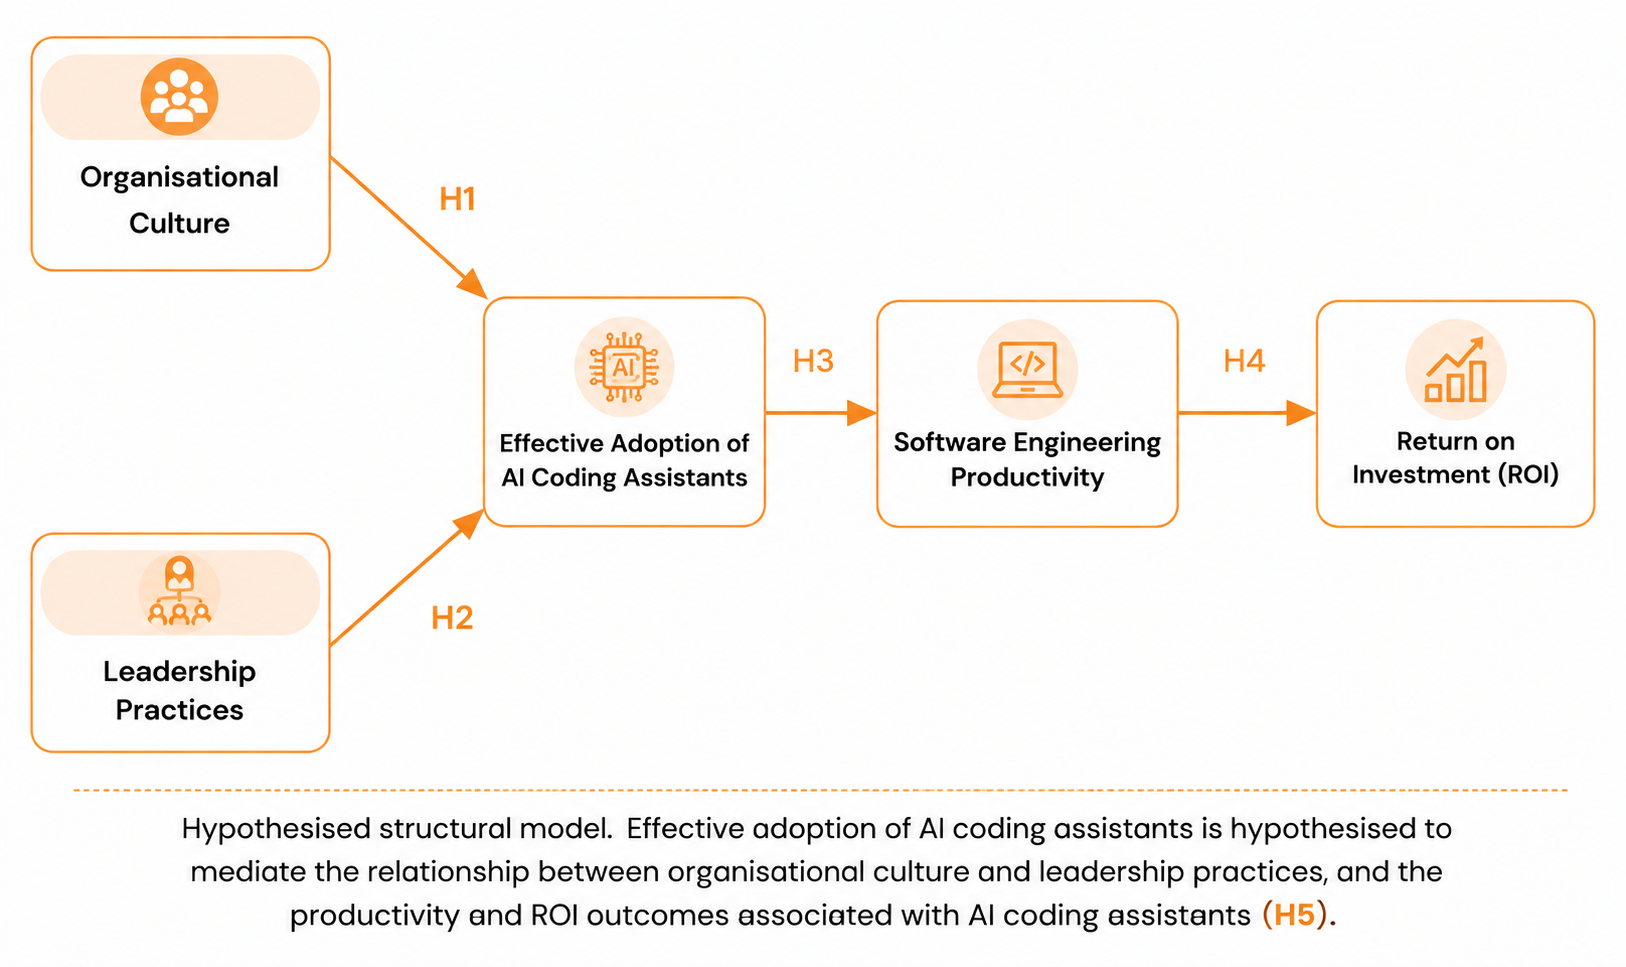
\includegraphics[width = 1\textwidth]{Images/Hypothesised_structural_model} % enter the filename here
		\caption{hypothesised model} % enter the figure caption here
		\label{fig:hypothesised_model} % enter the figure label here (for cross referencing)
	\end{center}
\end{figure}

Hypothesised model. Assimilation quality is hypothesised to mediate the relationship between organisational culture and AI leadership and governance support, and the ROI realised from AI coding assistants (H4). Organisational readiness, team size, developer experience, and adoption duration were entered as control variables with direct paths to ROI.

\section{Population and Sampling}
\label{sec:Population and Sampling}
\subsection{Target Population}
\label{sec:Target Population}
The study focused on software engineering teams within large organisations in South Africa that uses AI coding assistants.

\subsection{Sampling Strategy}
\label{sec:Sampling Strategy}
A purposive sampling strategy was adopted on this study, focusing on organisations that met the following criteria:
\begin{itemize}
	\item Used AI coding assistants;
	\item Had used AI coding assistants for at least six months; and
	\item Maintained measurable software engineering metrics.
\end{itemize}

The participants of the study comprised of software engineering professionals who worked in these organisations including developers, technical leads, and engineering managers, and who were selected using stratified sampling technique. 

Following the requirement of the methodological guidance, which states that there should be at least 200 in order to conduct correlation/SEM analysis for obtaining reliable and valid estimates \autocite{Hair2019}, the target sample size of this study was 250 to 300 participants. There were a total of 357 responses received, out of which 355 responses fulfilled the eligibility criteria of currently using AI coding assistants.

This minimum was corroborated after data collection using two established PLS-SEM sample-size heuristics, applied to the final analytical sample ($N=354$) and the largest number of predictors entered on a single construct in the structural model (seven, for ROI). The ten-times rule, which recommends at least ten observations per predictor on the most heavily predicted construct, implies a minimum of 70; the more formal inverse-square-root method \autocite{Kock2018}, which relates minimum sample size to the smallest structural path coefficient a study should be powered to detect at 5\% significance and 80\% power, implies a minimum of 275 to reliably detect a path as small as .15, and of 99 to detect a path as small as .25. The final analytical sample of 354 therefore exceeded both the ten-times-rule minimum and the inverse-square-root minimum for every path coefficient found to be statistically significant in Chapter Four (all of which exceeded .35 in magnitude), though it fell short of the inverse-square-root minimum needed to reliably detect a path as small as .12 (which would require $N=430$). Several of the non-significant control-variable paths reported in Chapter Four were smaller than this study was well powered to detect, so their non-significance should be read as inconclusive rather than as confident evidence of a true null effect.

\section{Measurement and Operationalisation}
\label{sec:Measurement and Operationalisation}
For each latent construct, measurement scales were created to ensure the construct validity \autocite{DeVellis2022}. A five-point Likert scale was used to measure each construct. As per the numeric coding system agreed for this analysis, responses were coded as 1 (Strongly Agree), 2 (Agree), 3 (Neither Agree nor Disagree), 4 (Disagree), and 5 (Strongly Disagree); for all items, the same direction was used, where a lower mean score means a stronger agreement. There is no influence of this coding option on the substantive conclusions obtained from the analysis; the reliability coefficients remain unaffected due to the uniform use of recording and the correlation or path coefficient of having two constructs coded in the same way showcases the same sign; it is stressed in this section and in chapter four as well to clarify the interpretation of means and skewness statistics.

\subsection{Organisational Culture}
\label{sec:Organisational Culture}
\textbf{Organisational culture} was assessed using adapted and validated scales addressing the following dimensions:

\begin{itemize}
	\item \textbf{Psychological Safety}
\end{itemize}
\textbf{Psychological safety} refers to the degree of comfort felt by members of a group to experiment, question, and contribute ideas without fear of criticism. In software engineering teams using AI coding assistants such as GitHub Copilot, psychological safety enables developers to question the suggestions generated by the tool. Developers who feel safe experimenting with the tool are better placed to become proficient in its use and to draw effectively on generative AI. Literature on the use of generative AI in knowledge work indicates that productivity gains are more pronounced where workers engage with such tools collaboratively \autocite{Noy2023}.

\begin{itemize}
	\item \textbf{Learning Orientation}
\end{itemize}
The \textbf{learning orientation} refers to how much the organisation values continual learning and development of skills. In an organisation that is implementing generative AI tools, the members will need to develop the necessary skills to work with these technologies effectively. Thus, organisations that have a strong learning orientation possess a higher chance to be able to implement generative AI successfully. Empirical studies show that generative AI has a high potential to increase productivity at work due to its application by employees' on their jobs \autocite{Brynjolfsson2025}.

\begin{itemize}
	\item \textbf{Knowledge Sharing}
\end{itemize}
\textbf{Knowledge Sharing} refers to the transfer of knowledge and skills among the members of a team. In teams utilising AI coding assistants, this generally involves the transfer of knowledge related to prompts, methods of debugging and best practices for applying the tool, which in turn allows the team to take advantage of generative AI. Empirical studies show that software development teams depend on such knowledge sharing to use the tools wisely \autocite{Sergeyuk2025}.

\begin{itemize}
	\item \textbf{Digital Openness}
\end{itemize}
\textbf{Digital openness} refers to the willingness of organisations and their people to accept new digital technologies. Organisations that display digital openness are more likely to accept generative AI tools and to adapt their processes accordingly. In software engineering, digital openness is likely to encourage the adoption of AI coding assistants and to support developers in exploring new ways of improving their productivity.

The organisational culture scale comprised seven items covering experimentation, knowledge sharing, learning orientation, collaboration, innovation support, responsible use, and the evaluation of measurable value, and was measured using the five-point Likert scale described above \autocite{Bryman2016}.

\subsection{AI Leadership and Governance Support}
\label{sec:AI Leadership and Governance Support}
AI leadership and governance support was assessed using a four-item scale covering the following dimensions:

\begin{itemize}
	\item \textbf{Executive Sponsorship}
\end{itemize}
\textbf{Executive sponsorship} refers to the degree to which leaders of the organisation advocate for the use of generative AIs and make it clear how they should be used in the development. When the top leaders show their support for AI programming assistants, it provides assurance to the employees' that this technology is of importance and meets the expectations of the organisation. Research in the field of the use of generative AI in complex processes has shown that workers feel more confident in using AI technologies with support from the organisation \autocite{Noy2023}. Research on the phenomenon of the use of AI has shown that executive sponsorship allows for the orderly adoption of new technologies across departments \autocite{Brynjolfsson2025}.

\begin{itemize}
	\item \textbf{Metric Alignment}
\end{itemize}
In this context, \textbf{metric alignment} is defined as the degree to which business leaders express the expected value that will come from using an AI coding assistant, in order to ensure that the performance expectations meet the objectives set before AI adoption. Studies on generative AI productivity show that organisational outcomes are realised only if performance indicators match AI usage efficiency and task accomplishment. The alignment of metrics involves business leaders indicating the expected benefits from the use of an AI coding assistant and simultaneously managing performance expectations in light of these benefits \autocite{Noy2023}.

\begin{itemize}
	\item \textbf{Resource Support}
\end{itemize}
\textbf{Resource support} is defined as the funding, know-how, and labour that must be allocated for successful implementation of AI solutions. For instance, the successful use of AI coding assistants requires investment in training developers, integration into software development environments as well as in infrastructure and constant analysis of the results of AI coding assistants' implementation. \textcite{Babina2024} states that companies would not benefit from using such tools without enough resource support.

\begin{itemize}
	\item \textbf{Governance Clarity}
\end{itemize}
\textbf{Governance clarity} refers to the extent to which leaders ensure that governance, risk, and quality concerns related to AI coding assistants are actively addressed. Generative AI tools such as Copilot carry significant governance implications for intellectual property, security, and software quality assurance, and organisations therefore need well-defined governance structures to frame the use of AI-generated code and to establish clear accountability. Research on AI governance has found that organisations with well-defined structures are better placed to manage technology risk while still realising the associated productivity benefits \autocite{Hradecky2022}.

\subsection{Assimilation Quality of AI Coding Assistants}
\label{sec:Assimilation Quality of AI Coding Assistants}
The quality of assimilation refers to the level to which coding assistants are integrated in the activities of a software engineer in a productive way as opposed to simply being installed. In this regard this concept encompasses how well the instruments are incorporated into daily workflow, the regularity of the usage, the extent to which AI-produced output is scrutinised and the degree to which the usage of the technology is in compliance with governance and quality assurance standards. Some empirical studies related to coding assistants reveal that they can boost developers productivity, although the magnitude of productivity increase depends on the degree of technology integration into the processes \autocite{Brynjolfsson2025}. The construct under discussion is based on the eight-item measure that addresses the following aspects:

\begin{itemize}
	\item \textbf{Workflow Integration}
\end{itemize}
\textbf{Workflow integration} relates to how AI coding assistants are incorporated into the existing development workflow and how they are integrated into collaboration efforts, like code review, testing, and documentation. The tools that are integrated into the existing workflow are most likely to be welcomed by developers. Research has found that using AI within established workflows leads to productivity gains compared to its disruptive nature \autocite{Brynjolfsson2025}.

\begin{itemize}
	\item \textbf{Usage Consistency}
\end{itemize}
\textbf{Usage consistency} means to what extent AI coding assistants are used in accordance with certain expectations and standards during the software creation process by the given team. Studies show that any form of generative AI will lead to better productivity results in the case of its consistent application \autocite{Noy2023}.

\begin{itemize}
	\item \textbf{Trust Calibration}
\end{itemize}
\textbf{Trust calibration} is the developers capacity to correctly trust AI-generated outputs. This is reflected in the extent of evaluation of AI-generated code suggestions during their previous review before using them in the development process. Studies on how human beings and AI interact have revealed that success largely depends on the ability to find this very balance \autocite{Noy2023}.

\begin{itemize}
	\item \textbf{Training and Governance Support}
\end{itemize}
The indicator refers to whether the developers have received sufficient training on using AI programming assistants successfully, as well as whether there is proper governance and quality control of using AI-powered functions on the site. AI programming has shown that deeper engagement with the usage of AI technology positively affects the efficiency of development and problem-solving \autocite{Brynjolfsson2025}.

\subsection{Return on Investment (ROI)}
\label{sec:Return on Investment Measurement}
ROI was operationalised as the perceived business value realised from AI coding assistants, following the perceptual approach to ROI measurement common in information systems research where direct financial data are not accessible to individual respondents \autocite{Hair2019}. A 15-item scale assessed ROI across three conceptual levels:

\begin{itemize}
	\item \textbf{Task-Level ROI}
\end{itemize}
Task-level ROI (five items) captures the extent to which AI coding assistants have improved individual developer productivity, reduced the time required to complete coding tasks, improved the efficiency of routine development tasks, contributed to improved software quality, and improved overall delivery performance at the level of individual work.

\begin{itemize}
	\item \textbf{Workflow-Level ROI}
\end{itemize}
Workflow-level ROI (four items) captures the extent to which AI coding assistants have improved the efficiency of the overall development workflow, contributed to improved software quality, reduced rework, and improved delivery performance at the level of the team's workflow.

\begin{itemize}
	\item \textbf{Firm-Level ROI}
\end{itemize}
Firm-level ROI (six items) captures the extent to which AI coding assistants have contributed to lower software development costs, faster time to market, innovation in software products or services, benefits that outweigh the costs of adoption, business value beyond individual coding tasks, and financial value that justifies the investment made.

Because the three ROI levels are conceptually related facets of the same underlying construct, all 15 items were retained and were tested both as a single overall reflective construct and as three separate dimensional constructs; the two specifications were compared using the measurement evidence reported in Chapter Four (Section~\ref{sec:Discriminant validity}), and the final representation used in the structural model was selected on that basis, in line with the principle that model specification should follow theory and measurement evidence rather than the significance of any resulting path \autocite{Hair2019}.

\subsection{Control Variables}
\label{sec:Control Variables}
Four control variables were entered into the structural model with direct paths to ROI, so that the core theoretical relationships could be interpreted net of contextual influences that plausibly affect perceived ROI independently of organisational culture, leadership, or assimilation quality.

Organisational readiness was measured using a six-item scale assessing whether the organisation has the technical infrastructure to support AI coding assistants, whether developers have the necessary skills, whether the organisation is generally ready to adopt and integrate AI technologies, whether adequate governance mechanisms are in place, whether the organisation is prepared to address associated risks (security, privacy, intellectual property, and quality), and whether it has the capability to assess whether AI coding assistants are generating measurable value. Unlike the remaining three control variables, organisational readiness was modelled as a reflective latent construct measured by its six items.

Team size, developer experience, and adoption duration were each measured using a single categorical item from the survey's screening section (team size in bands from fewer than five to more than twenty developers; professional development experience in bands from less than two years to more than ten years; and adoption duration in bands from less than six months to more than two years) and were entered into the structural model as observed, single-indicator control variables. Team size and developer experience were retained as two distinct observed characteristics rather than combined into a single construct, since they describe conceptually different aspects of a respondent's context.

\section{Data Collection}
\label{sec:Data Collection}
Data were collected through a structured online questionnaire administered via Google Forms. Online questionnaires are widely used in organisational and information systems research owing to their effectiveness in reaching dispersed samples. The questionnaire comprised closed-ended items measured using the five-point Likert scale described in Section~\ref{sec:Measurement and Operationalisation}, assessing organisational culture, AI leadership and governance support, the assimilation quality of AI coding assistants, ROI, and organisational readiness, together with a short screening and demographic section covering AI coding assistant use, adoption duration, role, team size, and professional development experience.

The survey was shared through professional networks, IT societies, and tech forums. The participation was voluntary, and prior to data gathering ethical approval was secured. Survey participants who indicated no usage of an AI coding helper were eliminated from one of the important parts of the survey and filtered out in the eligibility part of the analysis (Chapter Four, Section~\ref{sec:Data Screening and Sample Profile}).

The questionnaire items were adapted from measurement scales validated in prior studies, an approach intended to support the reliability of the data collected.

Prior research on AI adoption suggests that the success of AI tools depends not only on the technology itself, but on how individuals and organisations adopt and use it \autocite{Brynjolfsson2025}. Accordingly, the study measured both behavioural and organisational dimensions of AI use.

\subsection{Pilot Testing}
\label{sec:Pilot Testing}
Before the full deployment of the questionnaire, a small group of software engineering practitioners took part in piloting the questionnaire, but they were not included in the sample used in the main study. In the pilot study, we assessed the clarity, length, and face validity of the items in the questionnaire, and adjusted the questionnaire accordingly before sending it to the target sample. Testing a questionnaire in this fashion is recommended so that measurement error can be minimized and it also make it easier for respondents to understand the questionnaire \autocite{DeVellis2022}.

\section{Data Analysis}
\label{sec:Data Analysis}
Data analysis proceeded in two stages, following established PLS-SEM practice for combining preliminary screening with confirmatory structural modelling \autocite{Hair2019}.

\textbf{Stage one: data screening and preliminary analysis.} The eligibility criterion (current use of an AI coding assistant) was applied first and independently of any subsequent result, yielding 355 eligible responses from 357 submitted; complete-case analysis was then applied to the eligible sample, yielding a final analytical sample of 354 (Chapter Four, Section~\ref{sec:Data Screening and Sample Profile}). Descriptive statistics (mean, standard deviation, minimum, maximum, skewness, and kurtosis) were computed for every item and for each construct, to characterise the sample and to check for out-of-range values and restricted variance. Internal consistency was assessed using Cronbach's alpha for each construct, computed separately for AI leadership and governance support, organisational culture, assimilation quality, organisational readiness, the 15-item ROI scale as a whole, and each of the three ROI dimensions individually, together with corrected item-total correlations. Common method bias was assessed using two procedures, Harman's single-factor test and a full-collinearity variance inflation factor test \autocite{Kock2015}, given that all constructs were measured by self-report from the same respondents at the same point in time. Finally, Pearson correlations were computed among provisional construct mean scores as a preliminary, descriptive view of the relationships between constructs; as noted in Section~\ref{sec:Quantitative Explanatory Design}, these correlations were not treated as the final test of the hypotheses.

\textbf{Stage two: PLS-SEM measurement and structural model.} A reflective measurement model was estimated for AI leadership and governance support, organisational culture, assimilation quality, ROI, and organisational readiness, together with a structural model specifying organisational culture and AI leadership and governance support as predictors of assimilation quality, assimilation quality and the four control variables (organisational readiness, team size, developer experience, and adoption duration) as predictors of ROI, and organisational culture and AI leadership and governance support as additional direct predictors of ROI. Measurement model quality was assessed using indicator outer loadings (retaining loadings at or above .708 as strong indicator contributions), Cronbach's alpha, composite reliability (Dillon-Goldstein's rho), average variance extracted (AVE, retaining constructs at or above .50), and the Dijkstra-Henseler consistency reliability coefficient (rho\textsubscript{A}), computed directly from the fitted model's outer weights and indicator correlation matrix using Dijkstra and Henseler's (2015) closed-form estimator \autocite{Dijkstra2015}, so that internal consistency was assessed using all three complementary coefficients rather than composite reliability and Cronbach's alpha alone. Discriminant validity was assessed using three procedures: the heterotrait-monotrait ratio of correlations (HTMT), with values below .85 treated as strong evidence of discriminant validity, values between .85 and .90 treated as borderline, and a percentile bootstrap 95\% confidence interval computed for every HTMT ratio so that discriminant validity could be assessed inferentially and not only against a fixed point-estimate threshold \autocite{Hair2019}; the Fornell-Larcker criterion, comparing the square root of each construct's AVE against its correlation with every other construct; and an inspection of item cross-loadings, checking that every indicator correlated most strongly with its own construct. Because the theoretical framework identifies ROI at three levels, HTMT evidence was used, together with a comparison of the model estimated with a single overall ROI construct against a model estimated with task-, workflow-, and firm-level ROI as three separate constructs, to select the final ROI specification reported in Chapter Four, consistent with the principle that this choice should be justified by measurement evidence rather than by whichever specification produces more significant paths \autocite{Hair2019}.

Structural model collinearity was assessed using the variance inflation factor (VIF), with values below 5 treated as free of serious multicollinearity. Structural path coefficients, their standard errors, t-values, and 95\% confidence intervals were estimated using bootstrapping (2,000 resamples, percentile method, two-tailed test), with a path treated as statistically supported where its 95\% confidence interval excluded zero. Effect sizes (f\textsuperscript{2}) were computed for each structural predictor by comparing the coefficient of determination (R\textsuperscript{2}) of the full model with that of a model omitting the predictor concerned, and R\textsuperscript{2} and adjusted R\textsuperscript{2} were reported for assimilation quality and ROI. The mediating effect of assimilation quality proposed in H4 was tested using the specific indirect effect (the product of the relevant path from organisational culture, or AI leadership and governance support, to assimilation quality, and the path from assimilation quality to ROI), with its own bootstrapped 95\% confidence interval; the pattern of direct and indirect results was then classified as indirect-only mediation, complementary partial mediation, competitive mediation, or no support for mediation, following standard PLS-SEM mediation-classification criteria \autocite{Hair2019}. Predictive relevance was assessed for each ROI indicator using a ten-fold cross-validated procedure in the spirit of PLSpredict, comparing the prediction error of the structural model with that of a linear regression benchmark and reporting Q\textsuperscript{2}\textsubscript{predict} for each indicator. Two robustness checks were performed: a comparison of the structural model estimated with and without the four control variables, and a comparison of the primary model with a sensitivity model excluding respondents who selected the most positive response option on every substantive item, together with the standardised root mean square residual (SRMR) as a supplementary approximate model-fit statistic. Finally, an importance-performance map analysis (IPMA) was conducted for the four constructs with a path to ROI, combining each construct's total effect on ROI (importance) with its rescaled mean score (performance), to translate the structural results into a managerial prioritisation \autocite{Hair2019}.

The PLS-SEM computations reported in Chapter Four were carried out using a Python-based implementation of the partial least squares path modelling algorithm, rather than the SmartPLS software package; this is stated explicitly here, since the two produce results based on the same underlying algorithm but are not the same software. Every statistic reported in Chapter Four that is defined by a published closed-form formula, including rho\textsubscript{A}, HTMT, the Fornell-Larcker criterion, and cross-loadings, was computed directly from that formula and is reported on the same basis as it would be in SmartPLS. Statistics that depend on random resampling, the structural path bootstrap and the specific indirect effect bootstrap, will vary slightly between any two runs of either toolchain unless the same random seed is fixed in both; this is a general property of bootstrapping rather than a limitation specific to the toolchain used here, and is noted so that the precise decimal values reported in Chapter Four are not mistaken for exactly reproducible constants.

Collectively, this analytical strategy was designed to generate empirical evidence on how organisational culture and AI leadership and governance support are associated with the ROI realised from AI coding assistants, the extent to which this association is explained by how well the tools are assimilated into software engineering practice, and how robust these relationships are once organisational readiness, team size, developer experience, and adoption duration are accounted for.

\section{Research Limitations}
\label{sec:Research Limitations}
As with any study, several methodological limitations should be acknowledged. First, the cross-sectional design captured relationships among variables at a single point in time; correlation, structural path, and mediation analysis can establish the strength, direction, and statistical significance of an association, but cannot establish causality with the same confidence as a longitudinal or experimental design \autocite{Creswell2018}. Second, all constructs were measured using self-reported items completed by the same respondents, which introduces the possibility of common method bias and social desirability bias; this risk is assessed directly in Chapter Four using Harman's single-factor test, and is compounded by a pronounced ceiling effect in the responses (Chapter Four, Section~\ref{sec:Data Screening and Descriptive Statistics}), which a sensitivity analysis excluding the most extreme response pattern shows materially affects the size, though not the direction, of some structural estimates. Third, organisational culture and AI leadership and governance support were found to be empirically difficult to separate on the more stringent HTMT criterion, including on that criterion's own bootstrap confidence interval, although not on the more conservative Fornell-Larcker criterion (Chapter Four, Section~\ref{sec:Discriminant validity}); this limits the extent to which their independent, direct effects on ROI can be separated in the structural model, even though their combined association with ROI, operating through assimilation quality, is estimated with more precision. Fourth, the three ROI sub-scales (task-, workflow-, and firm-level) were found not to be empirically distinguishable from one another, which supported the decision to represent ROI as a single overall construct in the final structural model, but also means the study cannot speak to whether organisational culture, leadership, or assimilation quality relate differently to ROI at the task, workflow, or firm level. Fifth, the use of purposive and stratified sampling, while appropriate for reaching organisations meeting the study's inclusion criteria, limits the extent to which the findings can be generalised beyond large South African organisations with at least six months of experience using AI coding assistants; the achieved sample also included a broader range of software engineering roles than the developers and team leads originally targeted, which is addressed further in Chapter Four. Sixth, ROI was operationalised through perceptual indicators rather than direct financial data, which may not fully capture the financial return realised by participating organisations. Finally, the scope of the structural analysis itself was bounded in two specific ways, disclosed here as deliberate decisions rather than oversights: measurement invariance and a multigroup comparison across role or team size (MICOM and PLS-MGA) were not tested, although the achieved sample would support this as a natural extension; and unobserved heterogeneity, nonlinear effects, and endogeneity were not modelled, each being a legitimate, more advanced extension beyond the scope of a single master's-level study. These limitations are revisited in Chapter Five, alongside recommendations for future research.

\section{Ethical Considerations}
\label{sec:Ethical Considerations}
All ethical aspects were taken into account in this research. Participation in the survey was voluntary, and respondents were informed of the purpose of the research prior to completing the questionnaire. The participants were assured that their responses would be kept anonymous.

No details that could help in identifying the respondents were obtained. The results of this research were used solely for academic purposes and stored in a secure way according to ethical principles underlying social research.

\section{Summary}
\label{sec:Summary}
This chapter has presented the methodological approach adopted in the study. A quantitative design combining preliminary correlational screening with partial least squares structural equation modelling was used to investigate the relationships between organisational culture, AI leadership and governance support, the assimilation quality of AI coding assistants, and ROI, net of the influence of organisational readiness, team size, developer experience, and adoption duration. Data were collected through a structured online survey of software engineering practitioners, and statistical techniques, including reliability analysis, Pearson correlation, and a bootstrapped PLS-SEM measurement and structural model, were used to test the hypothesised relationships within the conceptual framework.

Through this methodology, the study sought to generate empirical evidence on the influence of organisational and leadership factors on the value realised from generative AI tools in software engineering. The following chapter presents the results of this analysis.


% ------------------------------------------------------------------------------
% Chapter 4
% ------------------------------------------------------------------------------
\chapter{Results} % enter the name of the chapter here
\label{cha:ch4_results} % enter the chapter label here (for cross referencing)

\section{Introduction}
\label{sec:Ch4 Introduction}
This chapter presents the results of the data analysis described in Chapter Three. The chapter follows the two-stage analytical strategy set out in Section~\ref{sec:Data Analysis}: it first reports the sample profile, data screening, descriptive statistics, reliability, common method bias, and preliminary Pearson correlations; it then reports the partial least squares structural equation model (PLS-SEM), covering the measurement model, discriminant validity, the choice of ROI specification, the structural model and hypothesis tests, effect sizes, the mediation test, control variable effects, predictive assessment, and robustness checks. The chapter closes with a summary table mapping each hypothesis to its outcome.

In this chapter, two conventions for reporting statistics will be used consistently. Firstly, all Likert-type items were assigned values, coded from 1 (Strongly Agree) to 5 (Strongly Disagree), where  \emph{lower} mean score indicates \emph{higher} levels of agreement, which is directed coding that differs from the more commonly used approach that recognizes higher scores as representative of higher agreement levels. Every mean reported below is interpreted with this direction in mind. Secondly, the PLS-SEM statistics reported in Sections~\ref{sec:Measurement Model}--\ref{sec:Robustness and Sensitivity Analysis} were computed using a Python-based implementation of the partial least squares algorithm rather than the SmartPLS software package; both implement the same underlying algorithm, and every statistic reported in this chapter, including the Dijkstra-Henseler consistency reliability coefficient (rho\textsubscript{A}), computed directly from the fitted model's outer weights and indicator correlation matrix using Dijkstra and Henseler's (2015) closed-form estimator \autocite{Dijkstra2015}, is reported alongside Cronbach's alpha and composite reliability (Dillon-Goldstein's rho) rather than in place of them.

\section{Data Screening and Sample Profile}
\label{sec:Data Screening and Sample Profile}
A total of 357 responses were submitted. Two respondents indicated that their team did not use an AI coding assistant and were excluded under the study's pre-specified eligibility criterion, leaving 355 eligible responses, consistent with the primary eligibility rule for this dataset. Among these 355 eligible responses, one respondent had a single missing value on a substantive item (a workflow-level ROI item); following the complete-case rule specified in Chapter Three, this respondent was excluded, yielding a final analytical sample of $N = 354$. This 354 arises from a missing-data exclusion applied after the primary eligibility rule, and not from any additional role-based exclusion. Table~\ref{tab:sample_flow} summarises this response flow.

\begin{table}[htbp]
	\centering
	\caption{Sample eligibility and participant flow}
	\label{tab:sample_flow}
	\begin{tabular}{lr}
		\hline
		\textbf{Stage} & \textbf{n} \\
		\hline
		Responses submitted & 357 \\
		Excluded: team does not use an AI coding assistant & $-2$ \\
		Eligible sample (primary rule) & 355 \\
		Excluded: incomplete response on a substantive item & $-1$ \\
		Final analytical sample & 354 \\
		\hline
	\end{tabular}
\end{table}

Table~\ref{tab:demographic_profile} summarises the demographic and usage profile of the final analytical sample. Respondents were predominantly software developers and senior developers, most commonly worked in teams of six to twenty engineers, most commonly had between two and ten years of professional development experience, and most commonly had used AI coding assistants for between one and two years.

\begin{table}[htbp]
	\centering
	\caption{Participant demographic and usage profile ($N = 354$)}
	\label{tab:demographic_profile}
	\resizebox{\linewidth}{!}{%
		\begin{tabular}{llrr}
			\hline
			\textbf{Characteristic} & \textbf{Category} & \textbf{n} & \textbf{Valid \%} \\
			\hline
			Role & Software Developer & 179 & 50.6 \\
			& Senior Developer & 92 & 26.0 \\
			& Technical Lead & 45 & 12.7 \\
			& Engineering Manager & 19 & 5.4 \\
			& Other roles (combined) & 19 & 5.4 \\
			\hline
			Team size & 6 -- 10 developers & 163 & 46.0 \\
			& 11 -- 20 developers & 86 & 24.3 \\
			& 1 -- 5 developers & 68 & 19.2 \\
			& More than 20 developers & 37 & 10.5 \\
			\hline
			Professional development experience & 2 -- 5 years & 154 & 43.5 \\
			& 6 -- 10 years & 133 & 37.6 \\
			& More than 10 years & 40 & 11.3 \\
			& Less than 2 years & 27 & 7.6 \\
			\hline
			AI coding assistant adoption duration & 1 -- 2 years & 197 & 55.6 \\
			& Less than 6 months & 76 & 21.5 \\
			& 6 -- 12 months & 73 & 20.6 \\
			& More than 2 years & 8 & 2.3 \\
			\hline
		\end{tabular}%
	}
\end{table}

No out-of-range values were found on any five-point item (all observed values fell between 1 and 5), and no evidence of exact duplicate submissions was identified from response timestamps.

\section{Descriptive Statistics}
\label{sec:Data Screening and Descriptive Statistics}
Table~\ref{tab:descriptives} reports descriptive statistics for each construct, computed as the mean of its constituent items. Every construct returned a low mean (all below 1.35 on the 1-to-5 scale) with pronounced positive skew and, in most cases, high kurtosis, indicating that the large majority of respondents selected ``Strongly Agree'' or ``Agree'' on almost every item, regardless of which construct was being measured. This pattern, a marked ceiling effect concentrated at the ``Strongly Agree'' end of the scale, is examined further in the common method bias assessment (Section~\ref{sec:Common Method Bias}) and tested directly in a dedicated sensitivity analysis (Section~\ref{sec:Robustness and Sensitivity Analysis}), which re-estimates the structural model after excluding the 247 of 354 respondents (69.8\%) who selected the most positive response option on every single substantive item.

\begin{table}[htbp]
	\centering
	\caption{Construct-level descriptive statistics ($N = 354$; scale 1 = Strongly Agree to 5 = Strongly Disagree)}
	\label{tab:descriptives}
	\resizebox{\linewidth}{!}{%
		\begin{tabular}{lrrrrrr}
			\hline
			\textbf{Construct} & \textbf{Mean} & \textbf{SD} & \textbf{Min} & \textbf{Max} & \textbf{Skewness} & \textbf{Kurtosis} \\
			\hline
			AI Leadership and Governance Support & 1.151 & 0.358 & 1.00 & 3.00 & 2.523 & 6.160 \\
			Organisational Culture & 1.139 & 0.338 & 1.00 & 3.00 & 2.456 & 5.413 \\
			Assimilation Quality & 1.254 & 0.487 & 1.00 & 4.00 & 2.151 & 5.558 \\
			ROI Overall (15 items) & 1.295 & 0.625 & 1.00 & 5.00 & 2.769 & 9.135 \\
			ROI Task-level (E1) & 1.271 & 0.604 & 1.00 & 5.00 & 3.199 & 13.230 \\
			ROI Workflow-level (E2) & 1.302 & 0.665 & 1.00 & 5.00 & 2.986 & 10.889 \\
			ROI Firm-level (E3) & 1.310 & 0.651 & 1.00 & 5.00 & 2.739 & 9.183 \\
			Organisational Readiness & 1.297 & 0.607 & 1.00 & 4.167 & 2.437 & 6.245 \\
			\hline
		\end{tabular}%
	}
\end{table}

\section{Reliability}
\label{sec:Reliability and Convergent Validity}
Table~\ref{tab:reliability} reports Cronbach's alpha and the range of corrected item-total correlations for each construct, computed separately for AI leadership and governance support, organisational culture, assimilation quality, organisational readiness, the 15-item ROI scale as a whole, and each of the three ROI dimensions. Every construct exceeded the conventional acceptability threshold of .70, and every corrected item-total correlation exceeded the conventional review threshold of .30 by a wide margin. Several constructs exceeded an alpha of .95, which, following the decision rule in Chapter Three, was inspected further rather than treated as automatically indicative of poor measurement; the inter-item correlations underlying these very high alphas are consistent with the extensive item redundancy already visible in the ROI sub-scale intercorrelations, and are discussed alongside the common method bias assessment below.

\begin{table}[htbp]
	\centering
	\caption{Reliability results ($N = 354$)}
	\label{tab:reliability}
	\resizebox{\linewidth}{!}{%
		\begin{tabular}{lrrr}
			\hline
			\textbf{Construct} & \textbf{Items} & \textbf{Cronbach's alpha} & \textbf{Item-total $r$ range} \\
			\hline
			AI Leadership and Governance Support & 4 & .878 & .652 -- .794 \\
			Organisational Culture & 7 & .963 & .821 -- .910 \\
			Assimilation Quality & 8 & .960 & .837 -- .875 \\
			ROI Overall (15 items) & 15 & .990 & .902 -- .958 \\
			ROI Task-level (E1) & 5 & .980 & .916 -- .958 \\
			ROI Workflow-level (E2) & 4 & .976 & .929 -- .954 \\
			ROI Firm-level (E3) & 6 & .977 & .908 -- .946 \\
			Organisational Readiness & 6 & .974 & .894 -- .934 \\
			\hline
		\end{tabular}%
	}
\end{table}

No item's removal was considered on reliability grounds alone: every corrected item-total correlation exceeded .65, well above the .30 review threshold, so there was no diagnostic basis for treating any single item as a weak indicator at this stage. The measurement model in Section~\ref{sec:Measurement Model} provides a second, independent check on indicator quality through outer loadings.

\section{Common Method Bias}
\label{sec:Common Method Bias}
Because all constructs were measured through self-report from the same respondents at the same point in time, common method bias was assessed using two independent procedures, following recommended practice for single-source survey designs \autocite{Hair2019}.

First, Harman's single-factor test was conducted: an unrotated principal component analysis was run on all 40 substantive items (AI leadership and governance support, organisational culture, assimilation quality, the 15 ROI items, and organisational readiness). Four components had an eigenvalue above 1, but the first unrotated factor alone accounted for 65.4\% of the total variance, well above the conventional 50\% threshold used to flag common method bias as a material concern.

Second, a full-collinearity variance inflation factor (VIF) test was conducted \autocite{Kock2015}, in which every construct (including the three single-indicator controls) was regressed on every other construct in the model, with a full-collinearity VIF at or below 3.3 taken as evidence that common method bias is unlikely to be a serious problem. Figure~\ref{fig:cmb_harman} summarises the Harman's single-factor result graphically, and Table~\ref{tab:full_collinearity_vif} reports the full-collinearity VIF results.

\begin{figure}[htbp]
	\centering
	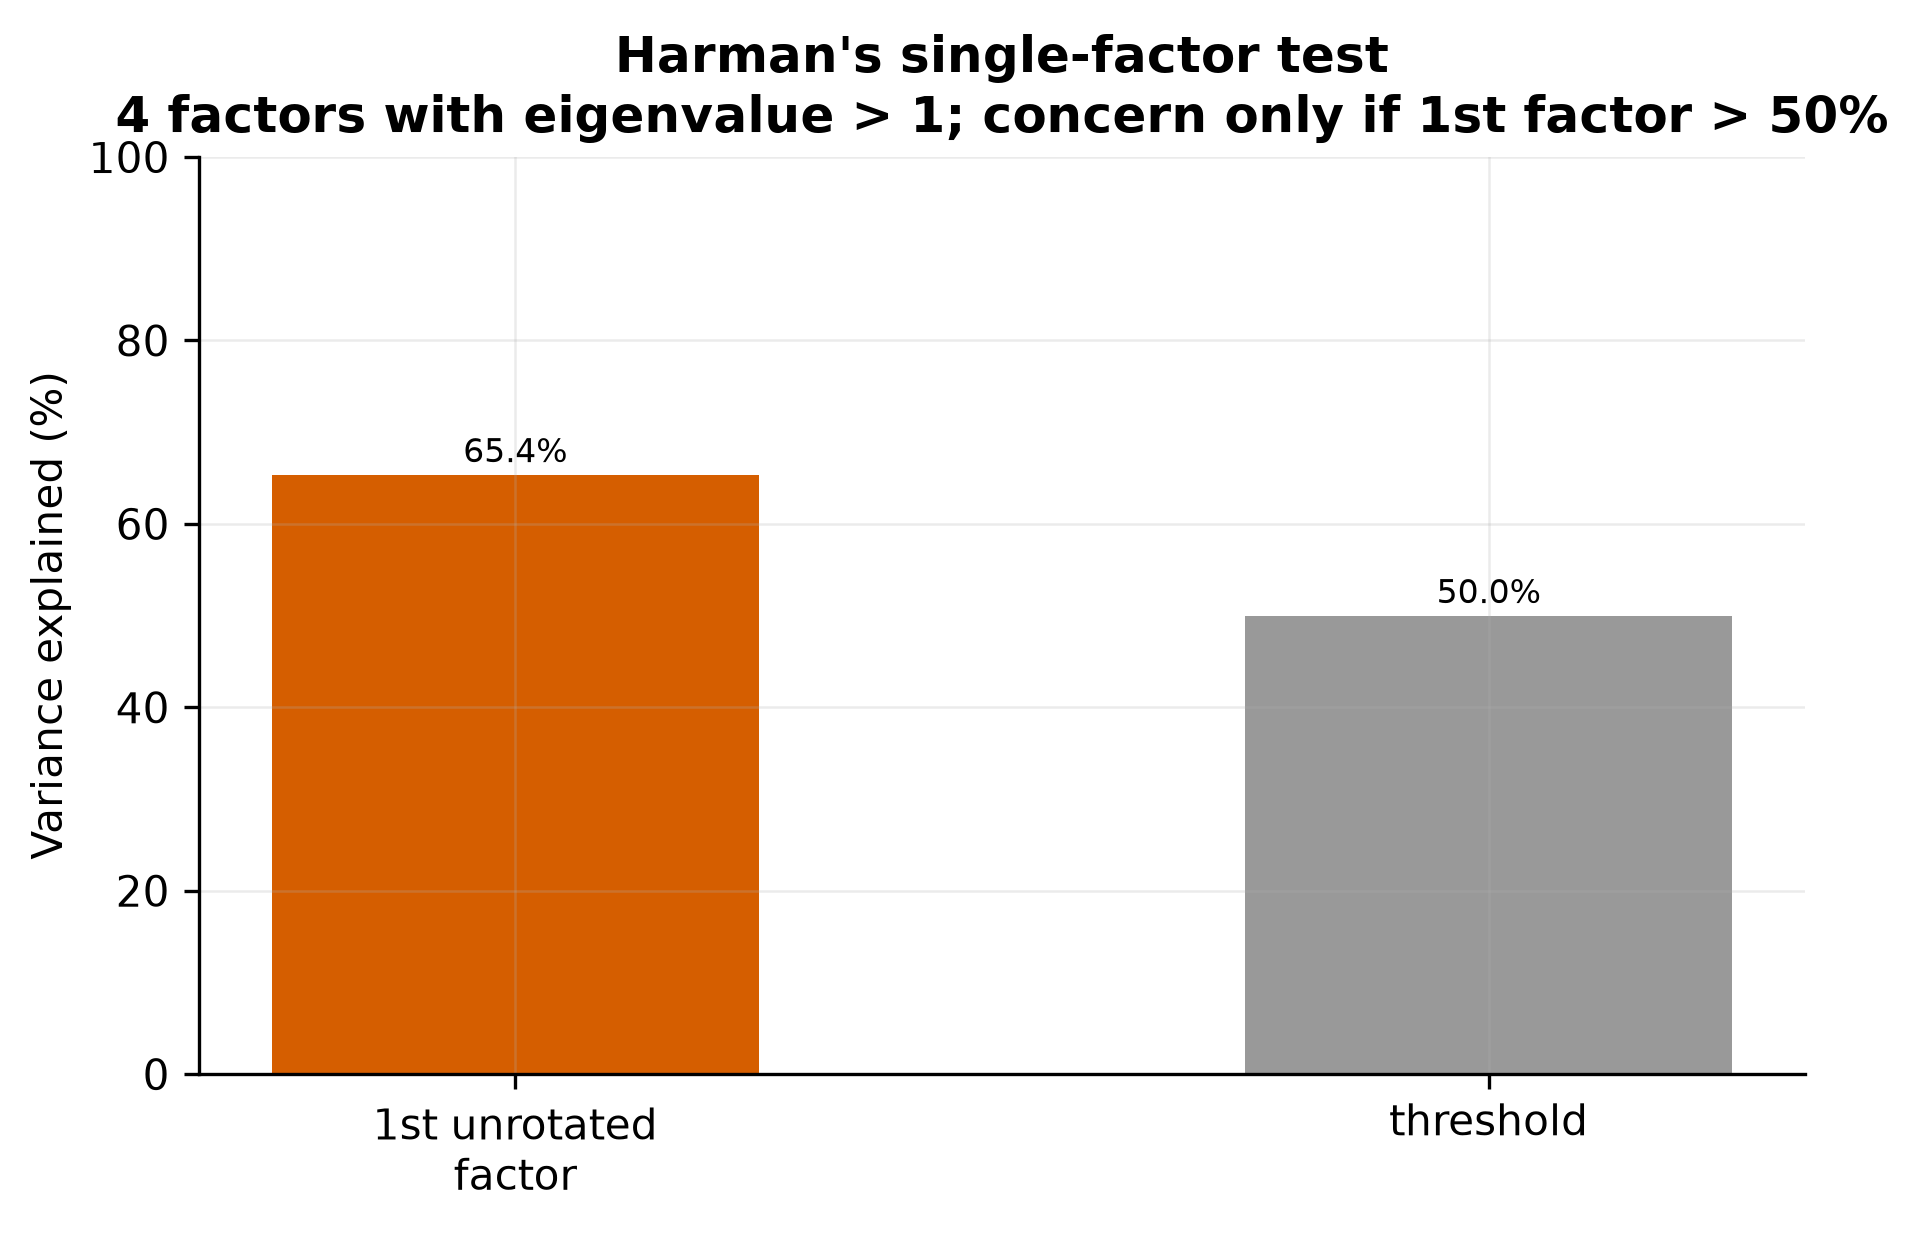
\includegraphics[width=0.75\linewidth]{Images/28_cmb_harman.png}
	\caption{Common method bias check: variance explained by successive unrotated principal components, with the first-factor threshold used by Harman's single-factor test.}
	\label{fig:cmb_harman}
\end{figure}

\begin{table}[htbp]
	\centering
	\caption{Full-collinearity VIF test for common method bias (Kock, 2015)}
	\label{tab:full_collinearity_vif}
	\begin{tabular}{lr}
		\hline
		\textbf{Construct} & \textbf{Full-collinearity VIF} \\
		\hline
		ROI & 5.422 \\
		Assimilation Quality & 5.035 \\
		Organisational Readiness & 4.846 \\
		Organisational Culture & 4.041 \\
		AI Leadership and Governance Support & 3.218 \\
		Developer Experience & 1.580 \\
		Team Size & 1.451 \\
		Adoption Duration & 1.115 \\
		\hline
	\end{tabular}
\end{table}

Five of the eight constructs, ROI, assimilation quality, organisational readiness, organisational culture, and AI leadership and governance support, exceeded the 3.3 threshold, with ROI itself reaching 5.422. Because this test is unrelated to the ceiling-effect analysis and does not simply restate the single-factor result, its agreement with Harman's test is informative rather than redundant: two different procedures, one based on the covariance structure of a single unrotated component and the other based on inter-construct collinearity, converge on the same conclusion. Common method bias is therefore treated as a genuine, and now doubly corroborated, concern for this dataset, to be borne in mind throughout the interpretation of the results that follow; it is revisited in the discussion of the structural model's discriminant validity (Section~\ref{sec:Discriminant validity}) and in Chapter Five.

\section{Preliminary Correlations}
\label{sec:Preliminary Correlations}
Following the reliability assessment, provisional mean scores were computed for each construct, and Pearson correlations were computed among them as a preliminary, descriptive step (Section~\ref{sec:Data Analysis}); these correlations are not the confirmatory test of the study's hypotheses, which is reported in Section~\ref{sec:Structural Model and Hypothesis Testing}. Table~\ref{tab:prelim_corr} reports the resulting correlation matrix; all coefficients were statistically significant at $p < .001$.

\begin{table}[htbp]
	\centering
	\caption{Preliminary Pearson correlations among provisional construct mean scores ($N = 354$, all $p < .001$)}
	\label{tab:prelim_corr}
	\resizebox{\linewidth}{!}{%
		\begin{tabular}{lrrrrrrrr}
			\hline
			& \textbf{Leadership} & \textbf{Culture} & \textbf{Assim.} & \textbf{ROI} & \textbf{E1} & \textbf{E2} & \textbf{E3} & \textbf{Readiness} \\
			\hline
			Leadership & 1.000 & & & & & & & \\
			Culture & 0.812 & 1.000 & & & & & & \\
			Assimilation Quality & 0.605 & 0.693 & 1.000 & & & & & \\
			ROI Overall & 0.446 & 0.531 & 0.830 & 1.000 & & & & \\
			ROI Task-level (E1) & 0.427 & 0.522 & 0.818 & 0.974 & 1.000 & & & \\
			ROI Workflow-level (E2) & 0.428 & 0.499 & 0.809 & 0.987 & 0.968 & 1.000 & & \\
			ROI Firm-level (E3) & 0.449 & 0.532 & 0.810 & 0.975 & 0.906 & 0.940 & 1.000 & \\
			Organisational Readiness & 0.440 & 0.505 & 0.812 & 0.877 & 0.851 & 0.855 & 0.866 & 1.000 \\
			\hline
		\end{tabular}%
	}
\end{table}

Two features of this matrix are notable in light of the discriminant validity results reported in Section~\ref{sec:Discriminant validity}. First, AI leadership and governance support and organisational culture were very highly correlated ($r = .812$). Second, the three ROI dimensions were correlated with one another at $r = .906$ to $.987$, and each was correlated with organisational readiness at $r = .851$ to $.866$, correlations high enough to raise a diagnostic concern about construct overlap (the manual's diagnostic trigger of $r > .80$), which is examined formally below.

\section{Measurement Model}
\label{sec:Measurement Model}
A reflective measurement model was estimated for AI leadership and governance support, organisational culture, assimilation quality, ROI, and organisational readiness, together with the three single-indicator control variables (team size, developer experience, and adoption duration). Table~\ref{tab:measurement_model} reports the range of outer loadings for each construct, together with Cronbach's alpha, composite reliability (Dillon-Goldstein's rho), and average variance extracted (AVE).

\begin{table}[htbp]
	\centering
	\caption{Measurement model: outer loadings, reliability, and convergent validity}
	\label{tab:measurement_model}
	\resizebox{\linewidth}{!}{%
		\begin{tabular}{lrrrrr}
			\hline
			\textbf{Construct} & \textbf{Loading range} & \textbf{Alpha} & \textbf{rho\textsubscript{A}} & \textbf{CR (Dillon-Goldstein)} & \textbf{AVE} \\
			\hline
			AI Leadership and Governance Support & .840 -- .879 & .885 & .896 & .921 & .740 \\
			Organisational Culture & .872 -- .932 & .964 & .970 & .970 & .822 \\
			Assimilation Quality & .859 -- .911 & .963 & .968 & .969 & .792 \\
			ROI Overall (15 items) & .909 -- .962 & .990 & .992 & .991 & .880 \\
			Organisational Readiness & .923 -- .955 & .975 & .976 & .980 & .889 \\
			\hline
		\end{tabular}%
	}
\end{table}

Every indicator loaded above .708 on its intended construct, the strong-loading threshold set out in Chapter Three, so no indicator was removed from the measurement model. Composite reliability exceeded .90 for every reflective construct (a level the review threshold in Chapter Three treats as a potential redundancy flag for constructs already showing an alpha above .95), and AVE exceeded .50 for every construct by a considerable margin (ranging from .740 for AI leadership and governance support to .889 for organisational readiness), indicating that each construct's indicators captured well over half of that construct's variance. rho\textsubscript{A} was computed directly from the fitted model's outer weights using Dijkstra and Henseler's (2015) closed-form estimator \autocite{Dijkstra2015} and fell, as expected, between Cronbach's alpha and composite reliability for every construct except ROI, whose three internal-consistency statistics (alpha $=.990$, rho\textsubscript{A}$=.992$, CR$=.991$) were effectively indistinguishable from one another to three decimal places, reflecting the extremely homogeneous, near-unidimensional response pattern already flagged for the 15-item ROI scale in Section~\ref{sec:Data Screening and Descriptive Statistics} and revisited in the common method bias assessment below. All three internal-consistency statistics, and rho\textsubscript{A} in particular, point to the same conclusion of strong, and for several constructs arguably redundant, internal consistency.

\section{Discriminant Validity}
\label{sec:Discriminant validity}
Discriminant validity was assessed using three procedures: the heterotrait-monotrait ratio of correlations (HTMT), with a bootstrapped confidence interval for every ratio; the Fornell-Larcker criterion; and an inspection of item cross-loadings. Table~\ref{tab:htmt} reports the HTMT matrix for the baseline model (with ROI represented as a single overall construct), together with the 95\% bootstrap confidence interval (percentile method, 2,000 resamples, fixed seed) for each ratio.

\begin{table}[htbp]
	\centering
	\caption{HTMT discriminant validity matrix, with bootstrap 95\% confidence intervals}
	\label{tab:htmt}
	\resizebox{\linewidth}{!}{%
		\begin{tabular}{llrrr}
			\hline
			\textbf{Pair} & & \textbf{HTMT} & \textbf{95\% CI lower} & \textbf{95\% CI upper} \\
			\hline
			Leadership & Culture & .881 & .776 & .967 \\
			Leadership & Assimilation Quality & .670 & .544 & .783 \\
			Leadership & ROI & .477 & .350 & .636 \\
			Leadership & Organisational Readiness & .475 & .347 & .616 \\
			Culture & Assimilation Quality & .728 & .637 & .808 \\
			Culture & ROI & .543 & .427 & .676 \\
			Culture & Organisational Readiness & .521 & .394 & .657 \\
			Assimilation Quality & ROI & .851 & .799 & .904 \\
			Assimilation Quality & Organisational Readiness & .841 & .756 & .916 \\
			ROI & Organisational Readiness & .895 & .816 & .951 \\
			\hline
		\end{tabular}%
	}
\end{table}

Most HTMT point estimates fell below the strong-evidence threshold of .85. Three values fell in the borderline range of .85 to .90: AI leadership and governance support versus organisational culture (HTMT $= .881$), assimilation quality versus ROI (HTMT $= .851$), and ROI versus organisational readiness (HTMT $= .895$); assimilation quality versus organisational readiness was just below this band (HTMT $= .841$). The bootstrap confidence intervals sharpen this picture in the way Hair et al. (2019) recommend \autocite{Hair2019}: every interval's upper bound remained below 1, so no pair of constructs can be said to be statistically indistinguishable from a single construct. However, for exactly these four pairs, leadership-culture, assimilation-ROI, assimilation-readiness, and ROI-readiness, the confidence interval's upper bound exceeded .90 (reaching as high as .967 for leadership-culture and .951 for ROI-readiness), meaning discriminant validity between these four pairs cannot be established with confidence even at the more lenient .90 threshold, only that the two constructs in each pair are not perfectly identical. For every other pair, the upper bound remained comfortably below .90, giving strong inferential, and not merely point-estimate, evidence of discriminant validity. Following the reporting template in Chapter Three, these results were not treated as invalidating the measurement model outright, but as identifying four specific pairs of constructs whose independent, discriminant contribution should be interpreted cautiously; this caution is reflected in the structural model results in Section~\ref{sec:Structural Model and Hypothesis Testing}, where AI leadership and governance support's direct effects are estimated with less precision than would be expected from its preliminary correlation with ROI, plausibly because a substantial part of what the leadership items measure overlaps with what the culture items measure, and in the discussion of organisational readiness's dominant effect in Chapter Five, which should be read alongside its borderline discriminant validity from both assimilation quality and ROI.

As a complement to HTMT, Table~\ref{tab:discriminant_fl} reports the Fornell-Larcker criterion: the square root of each construct's AVE on the diagonal, compared against its correlation with every other construct off the diagonal.

\begin{table}[htbp]
	\centering
	\caption{Fornell-Larcker discriminant validity matrix (diagonal = $\sqrt{\mathrm{AVE}}$)}
	\label{tab:discriminant_fl}
	\resizebox{\linewidth}{!}{%
		\begin{tabular}{lrrrrr}
			\hline
			& \textbf{Leadership} & \textbf{Culture} & \textbf{Assim.} & \textbf{ROI} & \textbf{Readiness} \\
			\hline
			Leadership & \textbf{.860} & & & & \\
			Culture & .817 & \textbf{.907} & & & \\
			Assimilation Quality & .608 & .689 & \textbf{.890} & & \\
			ROI & .453 & .533 & .830 & \textbf{.938} & \\
			Organisational Readiness & .445 & .505 & .810 & .877 & \textbf{.943} \\
			\hline
		\end{tabular}%
	}
\end{table}

By the Fornell-Larcker criterion, every construct's $\sqrt{\mathrm{AVE}}$ exceeded its correlation with every other construct, formally satisfying the criterion for all five constructs, including the four pairs flagged as borderline by the HTMT confidence intervals above (for example, ROI's $\sqrt{\mathrm{AVE}}$ of .938 exceeds its .877 correlation with organisational readiness, though only by .061). This divergence between HTMT and Fornell-Larcker is itself a well-documented property of the two criteria rather than a contradiction in the data: \textcite{Henseler2015} show that Fornell-Larcker is a comparatively conservative test that under-detects discriminant validity problems that HTMT is specifically designed to catch, which is why HTMT, not Fornell-Larcker, is treated as the primary discriminant validity criterion in this study, consistent with Chapter Three; the Fornell-Larcker result is reported as supplementary, corroborating evidence at the level the construct-correlation matrix can provide, not as evidence overriding the HTMT-based caution above.

Finally, cross-loadings were inspected for every one of the 40 substantive items: an item's correlation with its own (home) construct's score was compared against its correlation with every other construct's score. All 40 items loaded most strongly on their intended construct, so no item was flagged for possible mis-specification on this third discriminant validity criterion. The margin between an item's home-construct and next-highest cross-construct correlation varied considerably, from as little as .053 for one organisational readiness item up to .227 for one leadership item; the narrowest margins were concentrated among the organisational readiness and firm-level ROI items, consistent with the borderline HTMT evidence for the assimilation-ROI and ROI-readiness pairs reported above, while no item crossed over to load more strongly on a different construct than its own.

\subsection{ROI Specification: Overall Versus Dimensional}
\label{sec:ROI Specification}
Because the theoretical framework identifies ROI at three levels, task, workflow, and firm, a dimensional measurement model was also estimated, with task-level ROI (E1), workflow-level ROI (E2), and firm-level ROI (E3) specified as three separate reflective constructs. Table~\ref{tab:htmt_dimensional} reports the resulting HTMT values among the three dimensions and the remaining constructs.

\begin{table}[htbp]
	\centering
	\caption{HTMT discriminant validity: dimensional ROI specification}
	\label{tab:htmt_dimensional}
	\resizebox{\linewidth}{!}{%
		\begin{tabular}{lrrr}
			\hline
			& \textbf{Task ROI (E1)} & \textbf{Workflow ROI (E2)} & \textbf{Firm ROI (E3)} \\
			\hline
			Task ROI (E1) & -- & & \\
			Workflow ROI (E2) & .988 & -- & \\
			Firm ROI (E3) & .924 & .962 & -- \\
			\hline
		\end{tabular}%
	}
\end{table}

All three pairwise HTMT values among the ROI dimensions substantially exceeded the .90 threshold, indicating that task-, workflow-, and firm-level ROI could not be empirically distinguished from one another in this sample. The dimensional structural model (Table~\ref{tab:dimensional_paths}) told materially the same substantive story as the overall model, with very similar predictor patterns and only slightly lower explained variance for each dimension (task-level $R^2 = .780$; workflow-level $R^2 = .777$; firm-level $R^2 = .786$) than for the overall 15-item construct ($R^2 = .816$, Section~\ref{sec:Explanatory Power}). On the combined weight of this measurement evidence, the theoretical argument that a single underlying perceived-ROI construct is being expressed through three related item sets, and the requirement in Chapter Three that this choice be justified by evidence rather than by whichever specification yields more significant paths, the overall 15-item ROI construct was selected as the final specification reported in the structural model below. The dimensional model is retained here as supporting evidence for that decision and is not used for hypothesis testing.

\begin{table}[htbp]
	\centering
	\caption{Structural paths under the dimensional ROI specification (bootstrap, 2,000 resamples)}
	\label{tab:dimensional_paths}
	\resizebox{\linewidth}{!}{%
		\begin{tabular}{lrrrrr}
			\hline
			\textbf{Path} & \textbf{Task ROI $\beta$} & \textbf{Workflow ROI $\beta$} & \textbf{Firm ROI $\beta$} \\
			\hline
			Assimilation Quality $\rightarrow$ ROI dimension & .388$^{**}$ & .371$^{**}$ & .297$^{*}$ \\
			AI Leadership and Governance Support $\rightarrow$ ROI dimension & $-$.101 & $-$.046 & $-$.043 \\
			Organisational Culture $\rightarrow$ ROI dimension & .076 & .011 & .074 \\
			Organisational Readiness $\rightarrow$ ROI dimension & .544$^{***}$ & .568$^{***}$ & .606$^{***}$ \\
			Team Size $\rightarrow$ ROI dimension & .055 & .046 & .003 \\
			Developer Experience $\rightarrow$ ROI dimension & .062 & .076 & .056 \\
			Adoption Duration $\rightarrow$ ROI dimension & $-$.028 & $-$.028 & $-$.035 \\
			\hline
			\multicolumn{4}{l}{\footnotesize $^{*}p<.05$, $^{**}p<.01$, $^{***}p<.001$; coefficients are unstandardised PLS path coefficients on standardised indicators.}
		\end{tabular}%
	}
\end{table}

\section{Structural Model and Hypothesis Testing}
\label{sec:Structural Model and Hypothesis Testing}

\subsection{Collinearity}
\label{sec:Collinearity}
Inner variance inflation factors (VIF) were inspected before interpreting the structural path coefficients. Table~\ref{tab:vif} reports the results. All VIF values fell below the serious-collinearity threshold of 5; organisational culture and assimilation quality fell in the 3-to-5 range that Chapter Three treats as warranting cautious interpretation of individual coefficients, consistent with the high correlation between culture and leadership already noted.

\begin{table}[htbp]
	\centering
	\caption{Inner VIF for predictors of ROI, and of Assimilation Quality}
	\label{tab:vif}
	\resizebox{\linewidth}{!}{%
		\begin{tabular}{lr}
			\hline
			\textbf{Predictor of ROI} & \textbf{VIF} \\
			\hline
			Assimilation Quality & 4.474 \\
			Organisational Culture & 4.007 \\
			AI Leadership and Governance Support & 3.125 \\
			Organisational Readiness & 3.018 \\
			Developer Experience & 1.558 \\
			Team Size & 1.445 \\
			Adoption Duration & 1.115 \\
			\hline
			\textbf{Predictor of Assimilation Quality} & \textbf{VIF} \\
			\hline
			Organisational Culture & 2.940 \\
			AI Leadership and Governance Support & 2.940 \\
			\hline
		\end{tabular}%
	}
\end{table}

\subsection{Direct Effects and Hypothesis Testing}
\label{sec:Direct Effects}
Structural path coefficients were estimated with bootstrapping (2,000 resamples, percentile method, two-tailed test). Table~\ref{tab:structural_paths} reports the unstandardised path coefficient ($\beta$), bootstrap standard error, $t$-statistic, approximate $p$-value, and 95\% confidence interval for every path in the baseline (overall ROI) structural model.

\begin{table}[htbp]
	\centering
	\caption{Structural path coefficients (bootstrap, 2,000 resamples)}
	\label{tab:structural_paths}
	\resizebox{\linewidth}{!}{%
		\begin{tabular}{lrrrrr}
			\hline
			\textbf{Path} & \textbf{$\beta$} & \textbf{SE} & \textbf{$t$} & \textbf{$p$} & \textbf{95\% CI} \\
			\hline
			Organisational Culture $\rightarrow$ Assimilation Quality & .579 & .125 & 4.64 & $<.001$ & [.348, .820] \\
			AI Leadership and Governance Support $\rightarrow$ Assimilation Quality & .135 & .138 & 0.98 & .328 & [$-$.142, .385] \\
			Assimilation Quality $\rightarrow$ ROI & .356 & .147 & 2.43 & .015 & [.063, .624] \\
			Organisational Culture $\rightarrow$ ROI (direct) & .057 & .068 & 0.83 & .407 & [$-$.090, .194] \\
			AI Leadership and Governance Support $\rightarrow$ ROI (direct) & $-$.063 & .054 & $-$1.16 & .247 & [$-$.158, .051] \\
			Organisational Readiness $\rightarrow$ ROI & .588 & .135 & 4.35 & $<.001$ & [.344, .871] \\
			Team Size $\rightarrow$ ROI & .031 & .039 & 0.80 & .422 & [$-$.068, .074] \\
			Developer Experience $\rightarrow$ ROI & .065 & .047 & 1.36 & .173 & [$-$.076, .128] \\
			Adoption Duration $\rightarrow$ ROI & $-$.032 & .025 & $-$1.29 & .196 & [$-$.078, .019] \\
			\hline
		\end{tabular}%
	}
\end{table}

Three results bear directly on H1 to H3. First, organisational culture had a strong, statistically significant effect on assimilation quality, but its \emph{direct} effect on ROI, once assimilation quality and the four controls were included in the same model, was small and not statistically significant. Second, AI leadership and governance support's effect on assimilation quality, and its direct effect on ROI, were both small and not statistically significant. Third, assimilation quality had a statistically significant, positive direct effect on ROI. Because H1 and H2 concern the \emph{overall} association between each predictor and ROI, they were evaluated using the total effect (direct plus indirect via assimilation quality, Section~\ref{sec:Mediation Analysis Results}) rather than the direct effect alone; on that basis, H1 was supported (organisational culture's total effect on ROI was positive and, as shown below, its indirect component was statistically significant), while H2 was not supported (AI leadership and governance support's indirect effect was not statistically significant, and its direct effect was likewise not statistically significant, so no component of its total effect met the threshold for statistical support). This is a materially different conclusion from the preliminary Pearson correlation reported in Section~\ref{sec:Preliminary Correlations}, where both culture and leadership were significantly correlated with ROI; the structural model shows that, once the shared variance between culture and leadership and the four control variables are accounted for simultaneously, leadership's association with ROI does not hold up, illustrating directly why Chapter Three treats the preliminary correlations as screening evidence rather than as the confirmatory hypothesis test. H3 was supported: assimilation quality had a statistically significant, positive effect on ROI net of organisational culture, AI leadership and governance support, and all four controls.

Figure~\ref{fig:path_model} presents the estimated structural model in diagrammatic form, with each path's coefficient, significance, and the $R^2$ of each endogenous construct, to summarise the pattern described above at a glance.

\begin{figure}[htbp]
	\centering
	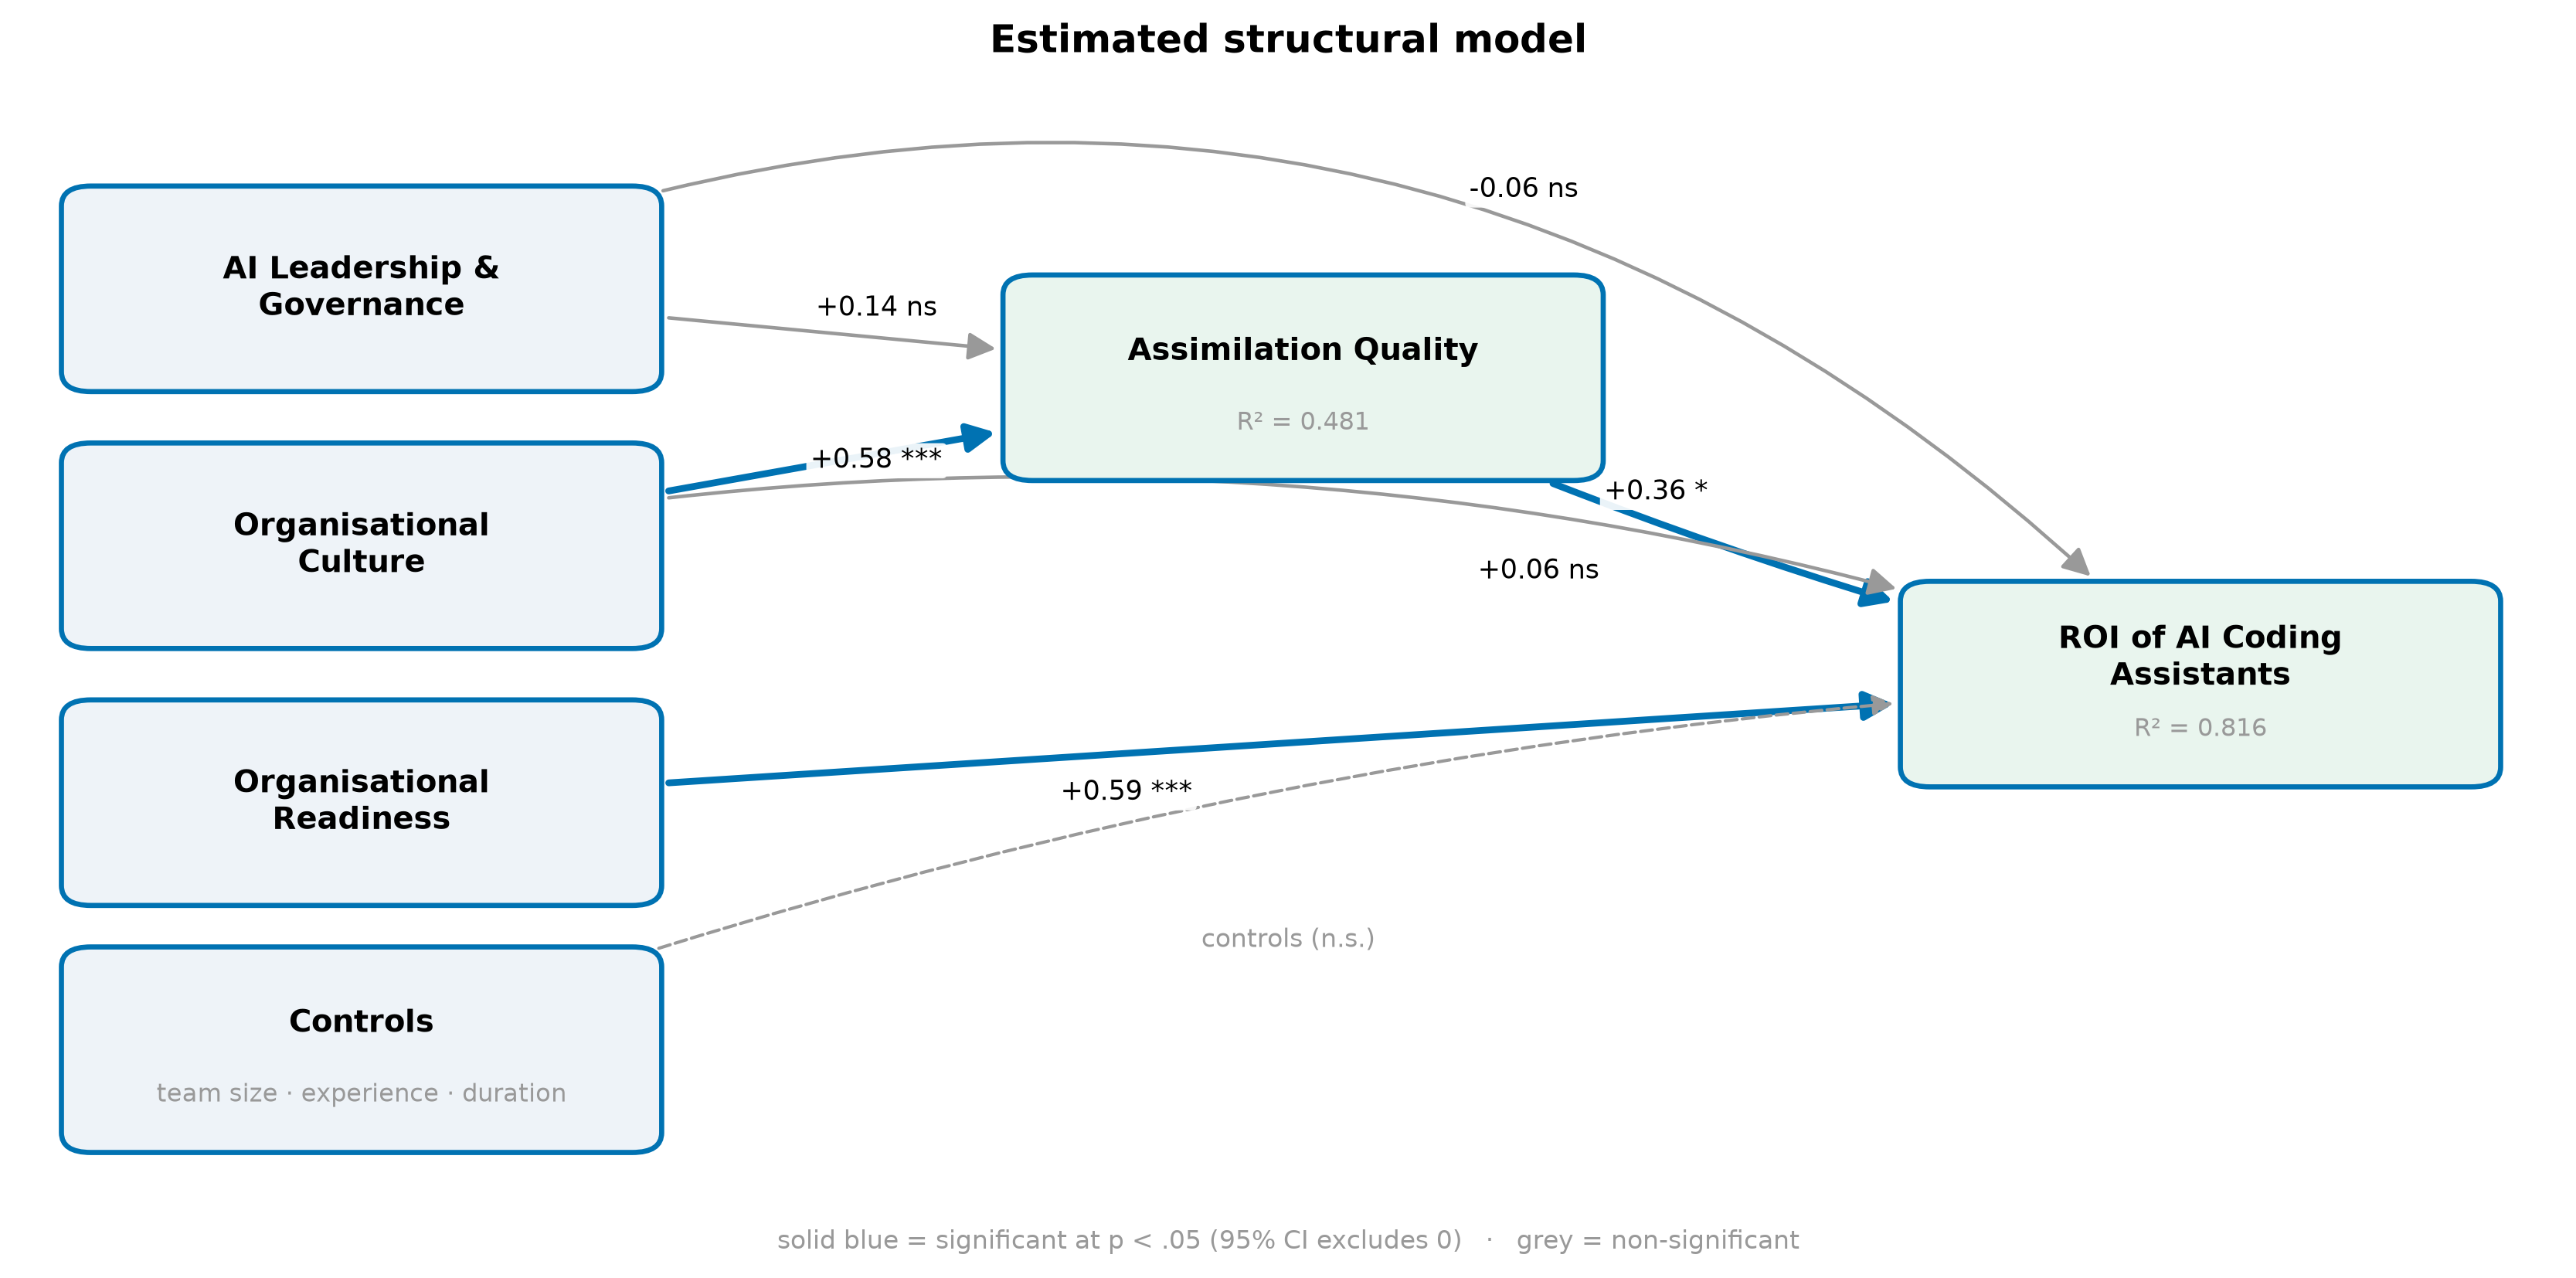
\includegraphics[width=\linewidth]{Images/17_path_model_diagram.png}
	\caption{Estimated structural model. Solid blue paths are statistically significant at $p<.05$ (95\% bootstrap confidence interval excludes zero); grey paths are not statistically significant.}
	\label{fig:path_model}
\end{figure}

\subsection{Explanatory Power and Effect Sizes}
\label{sec:Explanatory Power}
Table~\ref{tab:r2_f2} reports $R^2$, adjusted $R^2$, and $f^2$ effect sizes for the endogenous constructs.

\begin{table}[htbp]
	\centering
	\caption{$R^2$, adjusted $R^2$, and $f^2$ effect sizes}
	\label{tab:r2_f2}
	\resizebox{\linewidth}{!}{%
		\begin{tabular}{lrr}
			\hline
			\textbf{Endogenous construct} & \textbf{$R^2$} & \textbf{Adjusted $R^2$} \\
			\hline
			Assimilation Quality & .481 & .478 \\
			ROI & .816 & .812 \\
			\hline
			\textbf{Predictor of ROI} & \textbf{$f^2$} & \\
			\hline
			Organisational Readiness & .626 & (large) \\
			Assimilation Quality & .157 & (small-to-medium) \\
			Developer Experience & .015 & (negligible) \\
			Adoption Duration & .005 & (negligible) \\
			AI Leadership and Governance Support & .007 & (negligible) \\
			Team Size & .004 & (negligible) \\
			Organisational Culture & .004 & (negligible) \\
			\hline
			\textbf{Predictor of Assimilation Quality} & \textbf{$f^2$} & \\
			\hline
			Organisational Culture & .211 & (medium) \\
			AI Leadership and Governance Support & .011 & (negligible) \\
			\hline
		\end{tabular}%
	}
\end{table}

The structural model explained 48.1\% of the variance in assimilation quality and 81.6\% of the variance in ROI. The effect-size pattern reinforces the path-coefficient results: organisational readiness made, by a considerable margin, the largest individual contribution to explained variance in ROI ($f^2 = .626$, a large effect), ahead of assimilation quality ($f^2 = .157$), while organisational culture, AI leadership and governance support, and the three demographic controls each made a negligible direct contribution to ROI once the other predictors were held constant. For assimilation quality, organisational culture made a medium contribution ($f^2 = .211$) and AI leadership and governance support a negligible one ($f^2 = .011$), mirroring the path-coefficient pattern in Table~\ref{tab:structural_paths}.

\section{Mediation Analysis}
\label{sec:Mediation Analysis Results}
H4 proposed that assimilation quality mediates the relationship between (a) organisational culture and (b) AI leadership and governance support, and ROI. The specific indirect effect for each path was estimated as the product of the relevant path to assimilation quality and the path from assimilation quality to ROI, with its own bootstrapped 95\% confidence interval (2,000 resamples). Table~\ref{tab:mediation} reports the results, together with the direct effect for the same predictor and the resulting mediation classification, following the classification scheme in Chapter Three.

\begin{table}[htbp]
	\centering
	\caption{Specific indirect effects and mediation classification}
	\label{tab:mediation}
	\resizebox{\linewidth}{!}{%
		\begin{tabular}{lrrrrl}
			\hline
			\textbf{Path} & \textbf{Indirect $\beta$} & \textbf{95\% CI} & \textbf{Direct $\beta$} & \textbf{95\% CI} & \textbf{Classification} \\
			\hline
			Culture $\rightarrow$ Assimilation $\rightarrow$ ROI & .206$^{*}$ & [.025, .409] & .057 (ns) & [$-$.090, .194] & Indirect-only mediation \\
			Leadership $\rightarrow$ Assimilation $\rightarrow$ ROI & .048 (ns) & [$-$.057, .171] & $-$.063 (ns) & [$-$.158, .051] & No support for mediation \\
			\hline
			\multicolumn{6}{l}{\footnotesize $^{*}p<.05$; ns = not statistically significant (95\% CI includes zero).}
		\end{tabular}%
	}
\end{table}

For the organisational culture path, the indirect effect through assimilation quality was statistically significant (95\% CI excluded zero) while the direct effect was not, which the classification scheme in Chapter Three identifies as indirect-only mediation: culture's association with ROI in this sample operated through assimilation quality rather than through any additional direct channel. For the AI leadership and governance support path, neither the indirect effect nor the direct effect was statistically significant, so H4 was not supported for this path; assimilation quality cannot be said to mediate a relationship between leadership and ROI that was not itself established at either the direct or the indirect level. H4 was therefore partially supported: supported for the organisational culture pathway (H4a) and not supported for the AI leadership and governance support pathway (H4b).

\section{Control Variable Effects}
\label{sec:Control Variable Effects}
Table~\ref{tab:structural_paths} above reports the four control paths to ROI. Organisational readiness had, by a substantial margin, the strongest and most precisely estimated effect of any predictor in the model ($\beta = .588$, $p < .001$), exceeding even assimilation quality. None of team size, developer experience, or adoption duration had a statistically significant effect on ROI once the other predictors were included (all $p > .17$); developer experience showed the largest of the three coefficients, but its 95\% confidence interval still included zero. Because team size and developer experience are coded in ascending order (higher values indicating a larger team or more experience) while ROI retains the reversed Likert direction described in Section~\ref{sec:Ch4 Introduction}, a negative raw path coefficient corresponds to a positive association with perceived ROI and a positive raw coefficient corresponds to a negative association; applying this correction, adoption duration's coefficient ($\beta = -.032$, ns) corresponds to a small, statistically non-significant positive association between longer adoption duration and perceived ROI, and developer experience's coefficient ($\beta = .065$, ns) corresponds to a small, statistically non-significant negative association between greater developer experience and perceived ROI. None of these three associations reached statistical significance, and they are not interpreted further.

\section{Importance-Performance Map Analysis}
\label{sec:IPMA}
The path coefficients and effect sizes reported above establish which predictors matter statistically; they do not, on their own, indicate where managerial attention would be most productively directed, since a predictor's importance to ROI needs to be read alongside how well the organisation is already performing on that predictor. An importance-performance map analysis (IPMA) was therefore conducted for the four constructs with a hypothesised or control-variable path to ROI (organisational culture, AI leadership and governance support, assimilation quality, and organisational readiness), following standard PLS-SEM IPMA procedure \autocite{Hair2019}. Importance was operationalised as each construct's total standardised effect on ROI (direct effect plus, for culture and leadership, its indirect effect through assimilation quality); performance was operationalised by rescaling each construct's raw mean score (on the study's 1-to-5, Strongly-Agree-to-Strongly-Disagree scale) to a 0-to-100 index, where 100 represents the most positive possible score (a raw mean of 1, all ``Strongly Agree'') and 0 represents the least positive possible score (a raw mean of 5, all ``Strongly Disagree''). Table~\ref{tab:ipma} reports the results.

\begin{table}[htbp]
	\centering
	\caption{Importance-performance map analysis (target construct: ROI)}
	\label{tab:ipma}
	\resizebox{\linewidth}{!}{%
		\begin{tabular}{lrrr}
			\hline
			\textbf{Construct} & \textbf{Importance (total effect on ROI)} & \textbf{Mean (1--5 scale)} & \textbf{Performance (0--100)} \\
			\hline
			Organisational Readiness & .588 & 1.297 & 92.57 \\
			Assimilation Quality & .356 & 1.254 & 93.66 \\
			Organisational Culture & .262 & 1.139 & 96.52 \\
			AI Leadership and Governance Support & $-$.015 & 1.151 & 96.22 \\
			\hline
		\end{tabular}%
	}
\end{table}

Figure~\ref{fig:ipma} plots these results, with importance on the horizontal axis and performance on the vertical axis. Two features of the map are notable, and both reinforce conclusions reached elsewhere in this chapter through different evidence. First, organisational readiness combines the highest importance to ROI with the lowest performance score of the four constructs, placing it in the map's lower-right, ``priority for management action'' quadrant: it is simultaneously the construct ROI depends on most and the one on which respondents rated their organisations least positively, even though its absolute performance score (92.57) remains high in absolute terms given the ceiling effect that pervades this dataset. Second, AI leadership and governance support combines the lowest, and in fact a marginally negative, importance score with the second-highest performance score, placing it in the map's upper-left, ``high performance, low leverage'' quadrant; its near-zero importance reflects the total-effect calculation absorbing both its statistically non-significant direct effect on ROI and its statistically non-significant indirect effect through assimilation quality (Section~\ref{sec:Mediation Analysis Results}), so the negative sign should not be over-interpreted as evidence that leadership harms ROI, only that this study's structural model could not distinguish its total effect from zero. Because every item in this study is coded so that a lower raw score indicates stronger agreement, a positive importance value indicates that stronger agreement with a construct's items is associated with higher perceived ROI in the ordinary sense; this direction was confirmed for every construct's sign before interpreting the map. Read together with the effect-size results in Section~\ref{sec:Explanatory Power}, the IPMA provides a formal, quantified basis for the sequencing recommendation developed further in Chapter Five and Chapter Six: organisational readiness is both the most important and the least well-performing of the four constructs, making it the most defensible priority for managerial investment on this study's evidence.

\begin{figure}[htbp]
	\centering
	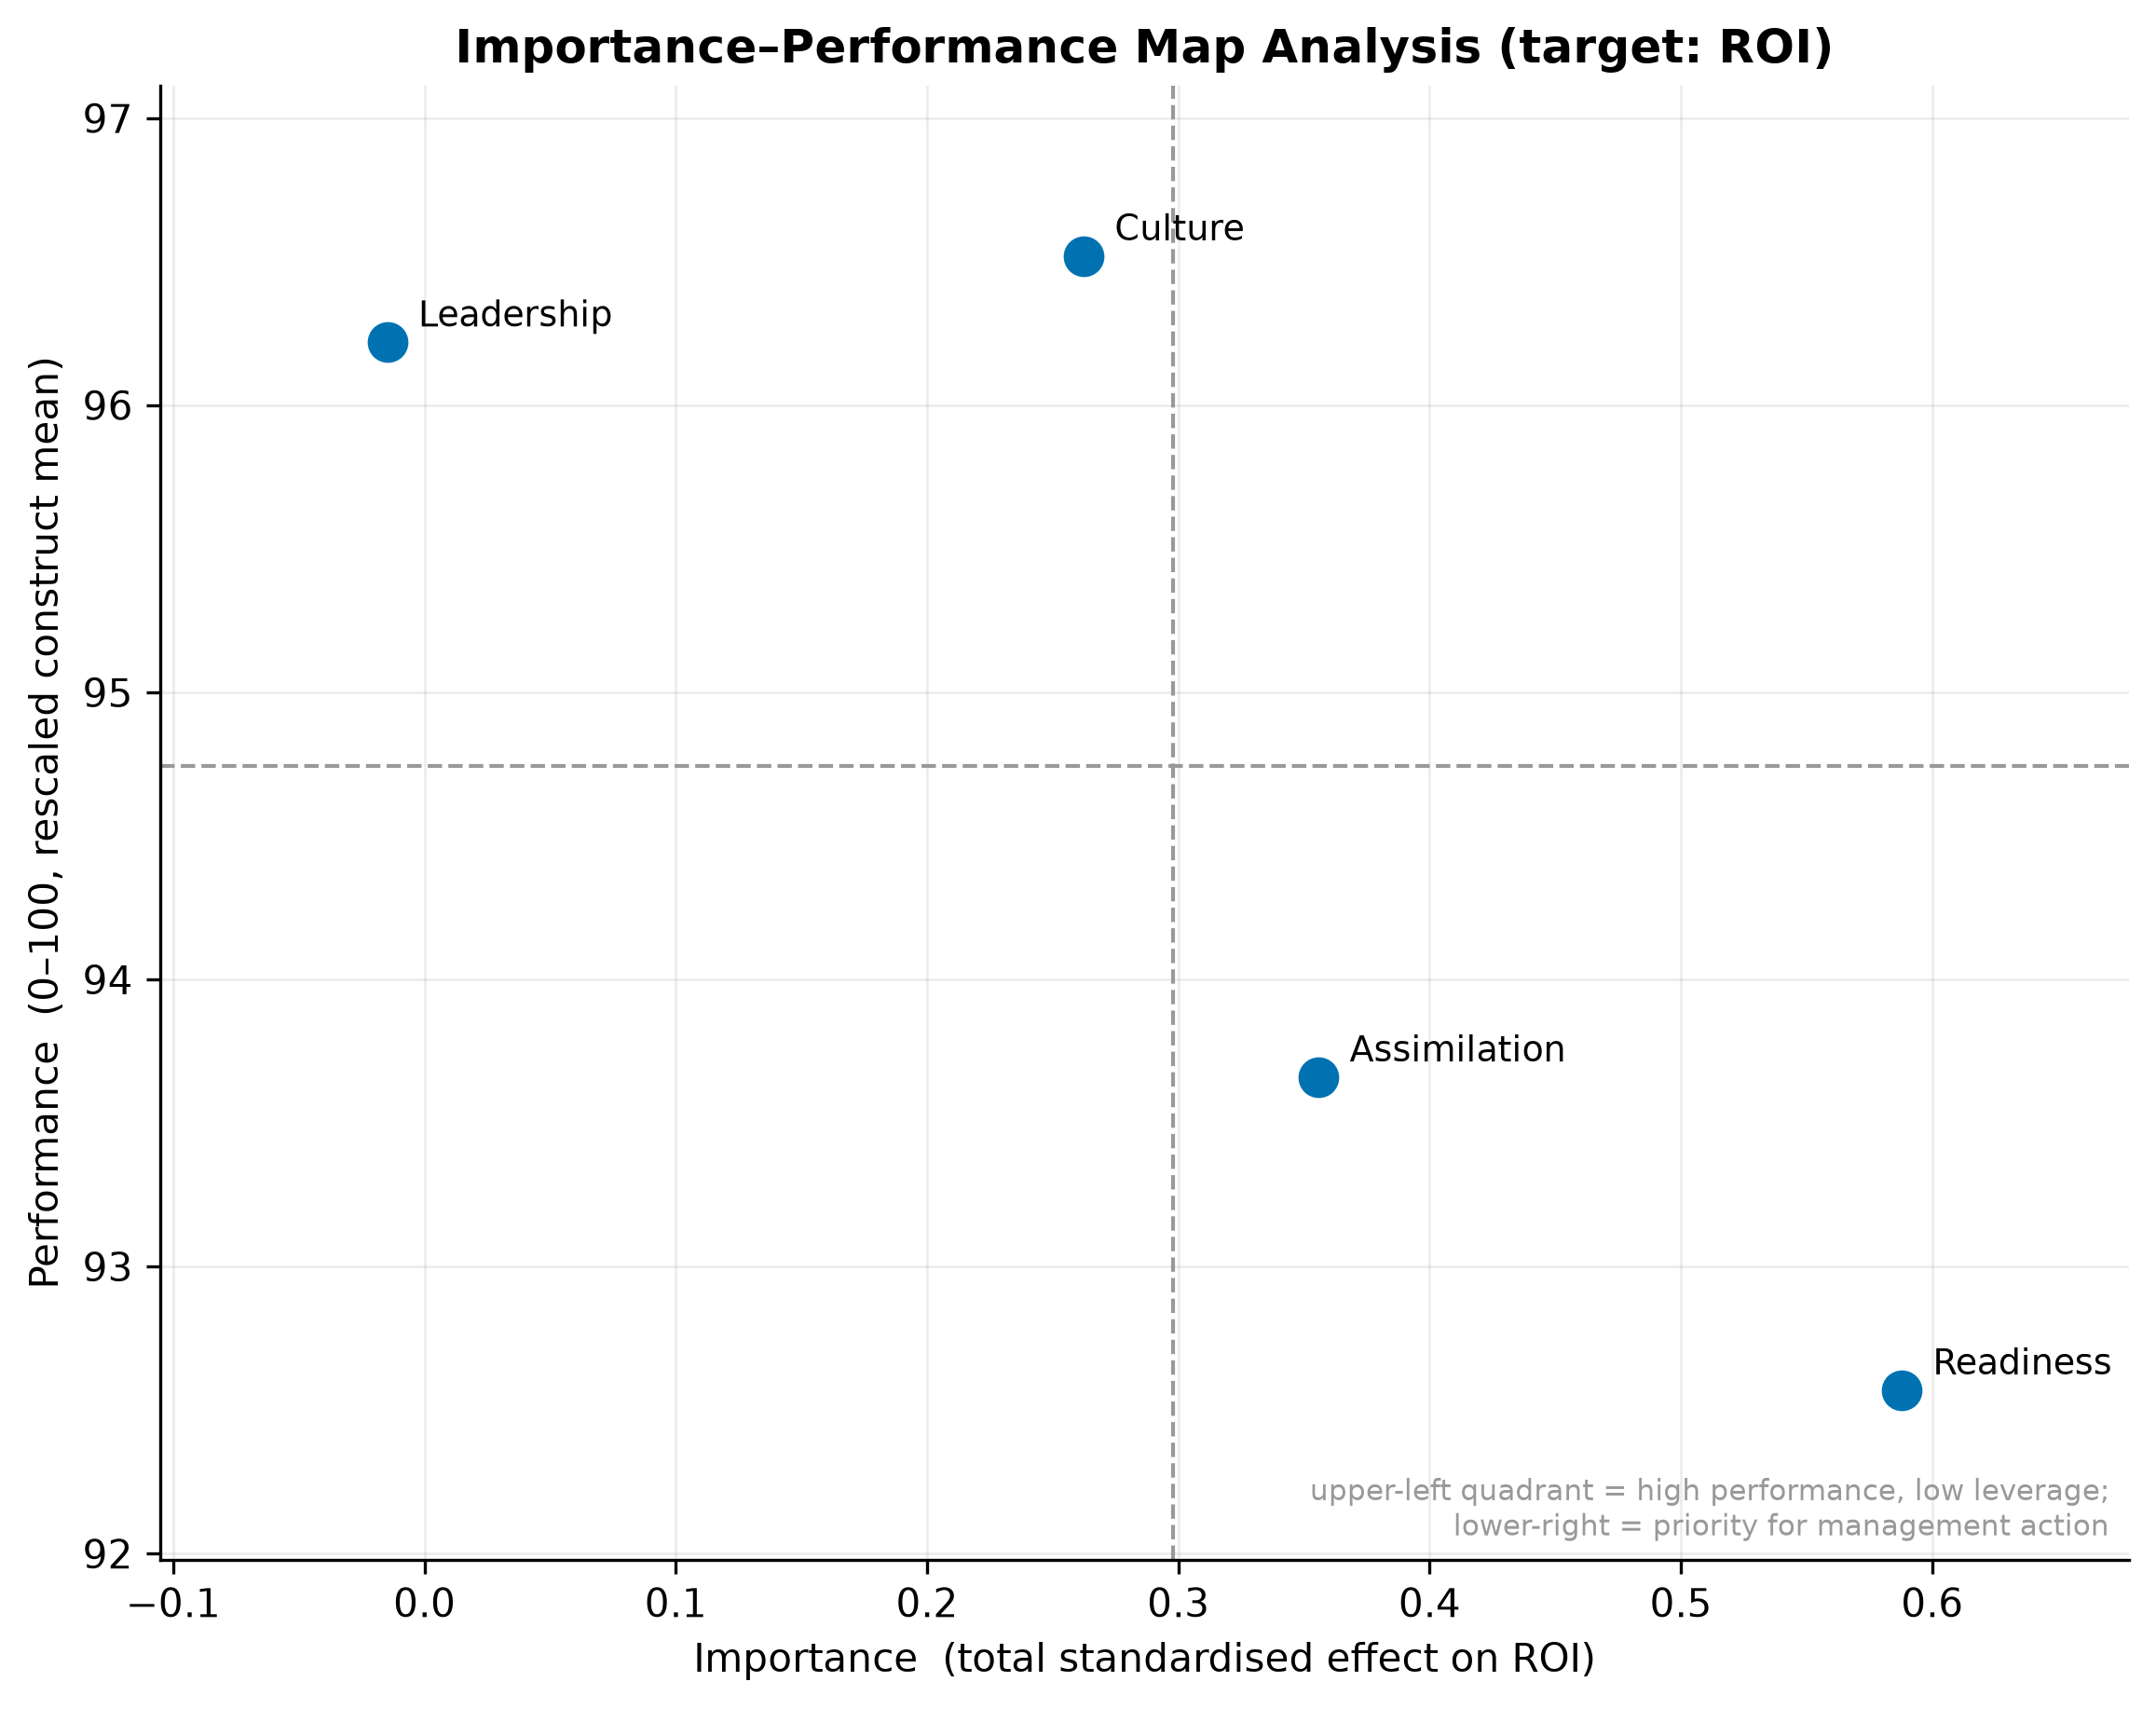
\includegraphics[width=0.8\linewidth]{Images/26_ipma.png}
	\caption{Importance-performance map for ROI. Lower-right quadrant (high importance, lower performance) indicates a priority for management action; upper-left (high performance, low importance) indicates a construct already performing well but with limited additional leverage over ROI.}
	\label{fig:ipma}
\end{figure}

\section{Supplementary Analysis: Individual Leadership Behaviours and ROI}
\label{sec:Leadership Behaviours Supplementary Analysis}
Research question 3 (Section~\ref{sec:Research questions}) asks which leadership behaviours most strongly affect ROI outcomes, a question about the relative contribution of the four specific behaviours, executive sponsorship, metric alignment, resource support, and governance clarity, rather than about the bundled four-item construct tested as a single predictor in H2. Because those four behaviours were measured with one item each (SL1 to SL4) and modelled as a single reflective construct in the structural model above, the structural test in Section~\ref{sec:Direct Effects} cannot, on its own, distinguish one behaviour's contribution from another's. To address RQ3 directly, this section reports the bivariate Pearson correlation between each individual leadership item and the overall ROI composite. This is a descriptive, item-level comparison rather than a further confirmatory structural test, and is reported as a supplementary analysis for this reason.

\begin{table}[htbp]
	\centering
	\caption{Individual leadership behaviours: correlation with ROI and PLS outer loading}
	\label{tab:leadership_items}
	\begin{tabular}{lrrr}
		\hline
		\textbf{Leadership behaviour (item)} & \textbf{$r$ with ROI} & \textbf{$p$} & \textbf{Outer loading} \\
		\hline
		Governance Clarity (SL4) & .431 & $<.001$ & .840 \\
		Executive Sponsorship (SL1) & .410 & $<.001$ & .853 \\
		Resource Support (SL3) & .360 & $<.001$ & .868 \\
		Metric Alignment (SL2) & .344 & $<.001$ & .879 \\
		\hline
	\end{tabular}
\end{table}

All four behaviours were significantly correlated with ROI at the item level ($p < .001$ in every case), and the differences between them were modest. Governance clarity, ensuring governance, risk, and quality concerns related to AI coding assistants are actively addressed, showed the strongest individual association with ROI ($r = .431$), followed closely by executive sponsorship ($r = .410$). Resource support ($r = .360$) and metric alignment ($r = .344$) showed somewhat weaker, though still significant, associations. This ordering is a useful, if modest, answer to RQ3: on this evidence, governance-related and visible-sponsorship behaviours showed a marginally stronger individual association with ROI than resourcing and metric-alignment behaviours did. It should not be over-interpreted, for two reasons. First, each behaviour was measured with a single item, so these correlations carry more measurement error than the multi-item constructs used elsewhere in this chapter, and a single item cannot separate a behaviour's true relationship with ROI from that item's own idiosyncratic wording. Second, and more importantly, this item-level comparison is a bivariate, preliminary analysis in the same sense as the correlations in Section~\ref{sec:Preliminary Correlations}: it does not control for organisational culture, assimilation quality, or the four control variables, all of which the confirmatory structural model in Section~\ref{sec:Direct Effects} shows matter a great deal to ROI. Given that the bundled, four-item leadership construct itself lost its significant association with ROI once modelled alongside culture (Section~\ref{sec:Direct Effects}), it is likely that these four individual item correlations would similarly attenuate if each behaviour were modelled as its own construct alongside the other predictors; testing that formally would require each behaviour to be measured with multiple items, which future research is recommended to pursue (Chapter Six).

\section{Predictive Assessment}
\label{sec:Predictive Assessment}
Predictive relevance was assessed for each of the 15 ROI indicators using a ten-fold cross-validated procedure in the spirit of PLSpredict, comparing the structural model's out-of-sample prediction error against a linear regression benchmark trained on the same exogenous indicators. Table~\ref{tab:predict} summarises the results.

\begin{table}[htbp]
	\centering
	\caption{Predictive assessment: Q\textsuperscript{2}\textsubscript{predict} and PLS-versus-linear-benchmark comparison}
	\label{tab:predict}
	\resizebox{\linewidth}{!}{%
		\begin{tabular}{lrl}
			\hline
			\textbf{ROI indicators} & \textbf{Q\textsuperscript{2}\textsubscript{predict} range} & \textbf{PLS RMSE vs.\ linear benchmark} \\
			\hline
			All 15 items & .511 to .626 & Mixed: PLS lower on 6 of 15 items \\
			\hline
		\end{tabular}%
	}
\end{table}

Every one of the 15 ROI indicators returned a $Q^2_{predict}$ value comfortably above zero, indicating that the structural model has predictive relevance for every indicator. The comparison against the linear benchmark, however, was mixed: the structural model achieved lower out-of-sample prediction error (RMSE) on 6 of the 15 indicators, while the linear benchmark achieved lower error on the remaining 9. Following the instruction in Chapter Three not to select only favourable indicators, this mixed result is reported as is; it is plausible given the very high inter-item correlations documented throughout this chapter, which mean that a simple linear combination of the raw exogenous items can predict individual ROI items about as well as the more parsimonious structural path model.

\section{Robustness and Sensitivity Analysis}
\label{sec:Robustness and Sensitivity Analysis}

\subsection{Model Fit}
\label{sec:Model Fit}
The standardised root mean square residual (SRMR), computed for the saturated measurement model across the five reflective constructs, was .054, below the .08 threshold conventionally viewed favourably in PLS-SEM.

\subsection{Control Sensitivity}
\label{sec:Control Sensitivity}
Table~\ref{tab:control_sensitivity} compares the core structural paths estimated with and without the four control variables.

\begin{table}[htbp]
	\centering
	\caption{Control sensitivity: core paths with and without controls}
	\label{tab:control_sensitivity}
	\resizebox{\linewidth}{!}{%
		\begin{tabular}{lrr}
			\hline
			\textbf{Path} & \textbf{With controls} & \textbf{Without controls} \\
			\hline
			Culture $\rightarrow$ Assimilation & .579 & .579 \\
			Leadership $\rightarrow$ Assimilation & .135 & .135 \\
			Assimilation $\rightarrow$ ROI & .356 & .363 \\
			Culture $\rightarrow$ ROI (direct) & .057 & .029 \\
			Leadership $\rightarrow$ ROI (direct) & $-$.063 & $-$.055 \\
			\hline
			$R^2$ (ROI) & .816 & .812 \\
			\hline
		\end{tabular}%
	}
\end{table}

The core theoretical paths were materially unchanged by the inclusion of the four control variables (all differences in the second decimal place), and $R^2$ for ROI changed by less than half a percentage point. The core model is therefore judged to be robust to the control specification; organisational readiness's substantial contribution to ROI (Section~\ref{sec:Explanatory Power}) is additional to, rather than a restatement of, the culture and assimilation-quality pathway.

\subsection{Response-Pattern Sensitivity}
\label{sec:Response-Pattern Sensitivity}
As noted in Section~\ref{sec:Data Screening and Descriptive Statistics}, 247 of the 354 respondents (69.8\%) selected the most positive response option, ``Strongly Agree'', on every single substantive item. Following Chapter Three, these respondents were retained in the primary analysis reported above, since uniformly positive responses are not, on their own, evidence of an invalid response; a sensitivity model was then estimated excluding them, leaving $n = 107$. Table~\ref{tab:straightline_sensitivity} compares the two models.

\begin{table}[htbp]
	\centering
	\caption{Response-pattern sensitivity: primary sample versus sample excluding uniformly positive respondents}
	\label{tab:straightline_sensitivity}
	\resizebox{\linewidth}{!}{%
		\begin{tabular}{lrr}
			\hline
			\textbf{Path} & \textbf{Primary ($N=354$)} & \textbf{Sensitivity ($n=107$)} \\
			\hline
			Culture $\rightarrow$ Assimilation & .579 & .403 \\
			Leadership $\rightarrow$ Assimilation & .135 & .020 \\
			Assimilation $\rightarrow$ ROI & .356 & .096 \\
			Culture $\rightarrow$ ROI (direct) & .057 & .156 \\
			Leadership $\rightarrow$ ROI (direct) & $-$.063 & $-$.137 \\
			Readiness $\rightarrow$ ROI & .588 & .749 \\
			\hline
			$R^2$ (Assimilation) & .481 & .174 \\
			$R^2$ (ROI) & .816 & .750 \\
			\hline
		\end{tabular}%
	}
\end{table}

Unlike the control sensitivity check, this comparison shows a material change in magnitude while confirming the model's direction: with the uniformly positive respondents excluded, every structural path retained its original sign, and the culture-to-assimilation path remained the dominant predictor of assimilation quality. The assimilation-quality-to-ROI path weakened substantially (from .356 to .096), $R^2$ for assimilation quality fell from .481 to .174, and $R^2$ for ROI fell from .816 to .750, while organisational readiness's effect on ROI strengthened further. This confirms that the mediation finding reported in Section~\ref{sec:Mediation Analysis Results} is directionally robust, but that its estimated strength in the primary model is inflated by the roughly two-thirds of the achieved sample who gave the most positive answer to every item. Following the instruction in Chapter Three to report such a change openly, this magnitude sensitivity is revisited in Chapter Five alongside the common method bias result, where it is treated as a boundary on the size, rather than the existence, of the assimilation-quality pathway.

\section{Summary of Results}
\label{sec:Summary of Results}
Table~\ref{tab:hypothesis_summary} summarises the outcome of each hypothesis.

\begin{table}[htbp]
	\centering
	\caption{Final hypothesis decision summary}
	\label{tab:hypothesis_summary}
	\resizebox{\linewidth}{!}{%
		\begin{tabular}{lp{9cm}l}
			\hline
			\textbf{Hyp.} & \textbf{Statement} & \textbf{Outcome} \\
			\hline
			H1 & Organisational culture $\rightarrow$ ROI (total effect) & Supported (indirect only; direct effect not significant) \\
			H2 & AI leadership and governance support $\rightarrow$ ROI (total effect) & Not supported \\
			H3 & Assimilation quality $\rightarrow$ ROI (direct effect) & Supported \\
			H4a & Assimilation quality mediates culture $\rightarrow$ ROI & Supported (indirect-only mediation) \\
			H4b & Assimilation quality mediates leadership $\rightarrow$ ROI & Not supported \\
			\hline
		\end{tabular}%
	}
\end{table}

Three findings stand out. First, once organisational culture and AI leadership and governance support were modelled simultaneously, alongside assimilation quality and the four control variables, only culture's association with ROI held up, and it did so entirely through assimilation quality rather than through any direct channel; leadership's preliminary correlation with ROI did not survive this more demanding test. Second, organisational readiness, entered as a control variable, emerged as the single strongest predictor of ROI in the model, ahead of assimilation quality itself. Third, a dedicated sensitivity analysis, prompted by the 69.8\% of respondents who selected the most positive response option throughout, confirmed that every structural path retained its direction when these respondents were excluded, though the assimilation-quality pathway in particular was found to be considerably smaller in that stricter sample; this boundary on the pathway's estimated strength should be read alongside the mediation and discriminant-validity findings discussed above. The following chapter discusses these results in relation to the literature reviewed in Chapter Two.

% ------------------------------------------------------------------------------
% Chapter 5
% ------------------------------------------------------------------------------
\chapter{Discussion} % enter the name of the chapter here
\label{cha:ch5_discussion} % enter the chapter label here (for cross referencing)

\section{Introduction}
\label{sec:Ch5 Introduction}
This chapter discusses the results presented in Chapter Four in relation to the literature reviewed in Chapter Two and the hypotheses formulated in Section~\ref{sec:Research Hypotheses}. The chapter is organised around the sample and data-quality picture, each hypothesis in turn, the unexpected prominence of organisational readiness as a control variable, the study's theoretical implications, its practical implications for IT leadership, and a summary.

\section{Discussion of the Sample and Response Pattern}
\label{sec:Discussion of the Sample}
The achieved sample of 354 software engineering practitioners was broader in role composition than the developers and team leads originally targeted in Section~\ref{sec:Sampling Strategy}, spanning software developers, senior developers, technical leads, engineering managers, and a small number of adjacent roles. This is a common feature of open, self-selected online surveys distributed through professional networks, and increases the range of perspectives captured, though it means the sample should be read as software engineering practitioners more broadly rather than strictly developers and team leads.

A more consequential feature of the data is the response pattern documented in Section~\ref{sec:Data Screening and Descriptive Statistics}: every construct, across all 354 respondents, returned a low mean with pronounced positive skew on the study's coding scale, and 247 respondents, 69.8\% of the sample, selected the most positive response option on every single substantive item. Combined with the very high reliability and composite reliability coefficients reported in Sections~\ref{sec:Reliability and Convergent Validity} and \ref{sec:Measurement Model}, the Harman's single-factor result reported in Section~\ref{sec:Common Method Bias} (65.4\% of variance on one unrotated factor), and the corroborating full-collinearity VIF result reported in the same section (five of eight constructs exceeding the conservative 3.3 threshold, ROI reaching 5.422), this pattern is most plausibly explained by a combination of two factors: a sample of practitioners who are, in the main, genuinely positive about their organisation's AI coding assistant journey, and a substantial degree of common method variance introduced by collecting all constructs from the same respondents, using the same response format, at the same time. That two conceptually distinct common-method-bias tests, one based on the variance explained by a single unrotated factor and the other based on inter-construct collinearity, converge on the same conclusion strengthens rather than merely repeats this reading of the data. The sensitivity analysis in Section~\ref{sec:Response-Pattern Sensitivity} gives this concern a concrete, quantified form rather than leaving it as a general caveat: when the 247 uniformly positive respondents were excluded, the path from assimilation quality to ROI fell from .356 to .096, and the variance explained in assimilation quality fell from 48.1\% to 17.4\%. The direction of every core relationship held, but a material part of its estimated strength in the primary analysis is attributable to the two-thirds of the sample who answered every item identically. The results below should accordingly be read as evidence of a strongly positive, internally consistent pattern of perception, whose statistical strength is inflated to a non-trivial and now-quantified degree by common method variance and ceiling effects.

\section{Discussion of the Direct Relationships}
\label{sec:Discussion of Direct Effects}

\subsection{H1: Organisational Culture and ROI}
\label{sec:Discussion H1}
The preliminary Pearson correlation between organisational culture and ROI was significant and moderately strong ($r = .531$, $p < .001$), consistent with the literature reviewed in Section~\ref{sec:Organizational Culture}, which argued that dimensions such as psychological safety, learning orientation, knowledge sharing, and digital openness create the conditions in which developers are willing to experiment with and trust generative AI tools \autocite{Noy2023}. The structural model in Section~\ref{sec:Structural Model and Hypothesis Testing}, however, shows that this association was carried almost entirely by an indirect pathway: culture's direct effect on ROI, once assimilation quality and the four control variables were included, was small and not statistically significant ($\beta = .057$, $p = .407$), while its indirect effect through assimilation quality was statistically significant ($\beta = .206$, 95\% CI [.025, .409]). H1 was therefore supported on the basis of the total effect, but the more precise, structural reading is that organisational culture matters for ROI specifically because, and to the extent that, it improves how well AI coding assistants are assimilated into engineering practice, not because of any separate, direct channel.

\subsection{H2: AI Leadership and Governance Support and ROI}
\label{sec:Discussion H2}
AI leadership and governance support was also significantly correlated with ROI at the preliminary stage ($r = .446$, $p < .001$), in line with prior research emphasising the role of executive sponsorship, governance clarity, resource support, and metric alignment in AI adoption outcomes \autocite{Brynjolfsson2025}. This association did not survive the structural model: neither leadership's direct effect on ROI ($\beta = -.063$, $p = .247$) nor its indirect effect through assimilation quality ($\beta = .048$, 95\% CI [$-$.057, .171]) was statistically significant, so H2 was not supported. The most plausible explanation lies in the discriminant validity results in Section~\ref{sec:Discriminant validity}: leadership and culture were correlated at $r = .812$, with an HTMT value of .881 whose bootstrap confidence interval upper bound (.967) remained above the .90 threshold, indicating that discriminant validity between the two constructs cannot be established with confidence and that a substantial part of what the leadership items capture overlaps with what the culture items capture. The Fornell-Larcker criterion did not flag this same pair as a concern, but this divergence is expected rather than contradictory: Fornell-Larcker is the more conservative of the two criteria, and HTMT is specifically designed to detect the kind of overlap present here \autocite{Henseler2015}, which is why the structural model result, not the Fornell-Larcker table, is treated as the decisive evidence on this point. Once both constructs were entered into the same model, culture, the stronger of the two individually, absorbed most of the shared explanatory power, leaving leadership's independent contribution statistically indistinguishable from zero. This does not mean leadership is unimportant in this sample; it means that, empirically, this study's leadership and culture items measured something that behaved as one largely overlapping construct rather than two clearly separable ones, and that whatever this combined construct contributes to ROI is better attributed, on the evidence here, to the culture measure. This result is a useful illustration, in its own right, of why Chapter Three distinguished a preliminary correlation from a confirmatory structural test: a predictor can correlate significantly with an outcome in isolation and still fail to show an independent effect once a closely related predictor is modelled alongside it.

Research question 3 asked, more specifically, which leadership behaviours most strongly affect ROI. The item-level supplementary analysis in Section~\ref{sec:Leadership Behaviours Supplementary Analysis} suggests a modest ordering, governance clarity and executive sponsorship showed the strongest individual bivariate associations with ROI, ahead of resource support and metric alignment, but this ordering should be read as a preliminary, single-item comparison rather than a confirmed structural finding, given that even the full four-item leadership construct did not retain an independent effect once organisational culture was included in the model. The most defensible answer this study can give to RQ3 is therefore a qualified one: among the leadership behaviours measured, governance-related and visible-sponsorship activity showed a marginally stronger individual association with ROI than resourcing or metric-alignment activity, but none of the four behaviours, individually or bundled, demonstrated an effect on ROI independent of organisational culture.

\subsection{H3: Assimilation Quality and ROI}
\label{sec:Discussion H3}
Assimilation quality had a statistically significant, positive direct effect on ROI in the structural model ($\beta = .356$, $p = .015$), supporting H3, and, together with organisational readiness, was one of only two predictors in the model with a confirmed independent effect on ROI. This is consistent with the view that installing an AI coding assistant is not sufficient to realise value from it; value follows from how well the tool is integrated into workflows, used consistently, appropriately trusted, and supported by adequate training and governance \autocite{Brynjolfsson2025}. The effect size for this path was small-to-medium ($f^2 = .157$), and, as discussed in Section~\ref{sec:Discussion of the Sample}, its estimated strength is sensitive to the ceiling-effect respondents; even in the more conservative sensitivity sample, however, the coefficient remained positive. Assimilation quality is therefore best read as a real, but more modest than the primary analysis alone suggests, direct contributor to ROI, and as the specific channel through which organisational culture's influence operates.

\section{The Prominence of Organisational Readiness}
\label{sec:Discussion Readiness}
The most striking result in Chapter Four was not one of the four hypothesised relationships but a control variable. Organisational readiness, entered as a control with a direct path to ROI, returned by far the strongest and most precisely estimated coefficient in the entire model ($\beta = .588$, $p < .001$, $f^2 = .626$, a large effect), exceeding assimilation quality's own effect on ROI by a considerable margin, and this result was robust both to the inclusion or exclusion of the other three controls (Section~\ref{sec:Control Sensitivity}) and, in direction and relative dominance, to the response-pattern sensitivity check (Section~\ref{sec:Response-Pattern Sensitivity}), where its coefficient strengthened further. Conceptually, organisational readiness captures whether the organisation has the technical infrastructure, developer skills, governance mechanisms, and risk and value-assessment capability to support AI coding assistants; the size of this effect suggests that, in this sample, having these foundational conditions in place was a more powerful predictor of perceived ROI than the assimilation-quality behaviours built on top of them. One interpretation consistent with the technology-adoption literature is that organisational readiness functions as a precondition: without adequate infrastructure, skills, and governance, the workflow-level behaviours captured by assimilation quality may simply not be achievable to the same degree, so readiness and assimilation quality could be capturing sequential rather than competing sources of value. The cross-sectional design of this study cannot adjudicate between that sequential interpretation and a simpler explanation, that readiness and ROI share substantial common-method variance as two of the most positively and uniformly rated constructs in the survey (Section~\ref{sec:Discussion of the Sample}); the HTMT value between readiness and ROI (.895) was itself in the borderline range for discriminant validity, and its bootstrap confidence interval upper bound (.951) remained above .90, so this finding should be read with that caveat attached, alongside the equally borderline HTMT evidence between readiness and assimilation quality (.841, CI upper bound .916). Even allowing for that caveat, the magnitude and robustness of the readiness effect is large enough that it should not be treated as a peripheral control result. The importance-performance map analysis reported in Section~\ref{sec:IPMA} puts a number on this conclusion rather than leaving it as an inference from the path coefficient alone: organisational readiness combined the highest total effect on ROI of the four constructs examined with the lowest performance score, placing it uniquely in the map's priority-for-action quadrant, while AI leadership and governance support combined the lowest importance with a high performance score, the opposite pattern. It is arguably the chapter's single most important finding for IT leadership practice, addressed further in Section~\ref{sec:Practical Implications for IT Leadership}.

\section{Discussion of the Mediating Role of Assimilation Quality}
\label{sec:Discussion H4}
Hypothesis H4 proposed that assimilation quality mediates the relationship between organisational culture and AI leadership and governance support, and ROI. This was supported for the organisational culture pathway and not supported for the AI leadership and governance support pathway (Section~\ref{sec:Mediation Analysis Results}). For the culture pathway, the pattern, a significant indirect effect and a non-significant direct effect, is what Chapter Three's classification scheme identifies as indirect-only mediation: organisational culture's association with ROI in this sample operated entirely through the quality with which AI coding assistants were assimilated into engineering practice, with no additional, separate channel of influence. For the leadership pathway, neither the direct nor the indirect effect was statistically significant, so the data provide no empirical support for a mediated relationship running through leadership at all; as discussed under H2, this most plausibly reflects the substantial overlap between the leadership and culture measures rather than a genuine absence of any leadership influence on ROI. Substantively, the clearest and most defensible conclusion the structural model supports is that culture contributes to ROI almost entirely by improving how well AI coding assistants are assimilated into engineering practice, that this indirect pathway is the dominant one recovered in the data, and that its estimated size should be read alongside the response-pattern sensitivity result in Section~\ref{sec:Response-Pattern Sensitivity}, which shows this pathway weakens considerably, while remaining positive, once the most uniformly positive respondents are excluded.

\section{Theoretical Implications}
\label{sec:Theoretical Implications}
Collectively, these findings extend post-positivist, technology-adoption-oriented accounts of generative AI in software engineering in three ways. First, they position organisational culture's influence on ROI as channelled specifically through assimilation quality rather than exercised directly, adding empirical specificity to prior work showing that productivity gains from generative AI tools depend on how effectively individuals and organisations integrate the technology into their work \autocite{Brynjolfsson2025,Noy2023}. Second, they show that a leadership construct closely related to culture can lose its apparent explanatory power once tested alongside culture in a single structural model, which is a caution for future studies in this area that measure leadership and culture as separate constructs without also checking their discriminant validity. Third, and more novel, they suggest that organisational readiness, foundational infrastructure, skills, and governance capability, may deserve a more central theoretical position in models of AI-driven ROI than the largely behavioural, assimilation-focused framing common in this literature; this study's own design, treating readiness only as a control, likely understates the theoretical attention this construct warrants, and future models could usefully treat organisational readiness as a first-order antecedent or moderator rather than a covariate. Finally, the very high inter-construct correlations, the borderline-to-weak discriminant validity between several conceptually related pairs, and the Harman's single-factor result underline a broader methodological point: self-report, single-source designs in this domain are at meaningful risk of common method variance and ceiling effects, and future theoretical work would benefit from designs that separate the measurement of organisational antecedents from the measurement of outcomes, or that supplement self-report with objective indicators.

\section{Practical Implications for IT Leadership}
\label{sec:Practical Implications for IT Leadership}
Given the dissertation's focus on the role of IT leadership in realising ROI from AI coding assistants, these findings carry three practical implications, in descending order of the empirical support behind them. First, and most strongly supported, IT leaders should treat organisational readiness, technical infrastructure, developer skills, governance mechanisms, and the capability to assess AI-generated value, as a foundational, high-priority investment area, since it was the strongest and most robust predictor of perceived ROI in this study, ahead of assimilation-quality behaviours themselves, and the importance-performance map analysis (Section~\ref{sec:IPMA}) places it uniquely in the quadrant combining the highest importance to ROI with the lowest relative performance of the four constructs examined, the formal definition of a management priority in this technique. Second, IT leaders seeking ROI from AI coding assistants should prioritise assimilation quality, workflow integration, consistent usage, appropriate trust and review of AI-generated output, and adequate training and governance support, since it showed a statistically supported, if more modest than initially apparent, direct association with ROI, and was the specific channel through which a supportive culture translated into value. Third, the findings counsel caution rather than a strong practical recommendation regarding leadership and governance activity in isolation from culture and readiness: sponsorship, metric alignment, resource support, and governance clarity did not show an independent, statistically supported association with ROI once modelled alongside organisational culture, which the discriminant validity results suggest is because the two were measured as substantially overlapping constructs in this sample rather than because leadership activity is unimportant; IT leaders should therefore not conclude that visible sponsorship and governance effort do not matter, but this study cannot show, on its own terms, that they matter independently of a supportive culture. Finally, given the very high and uniformly positive scores across the sample, and the common-method-bias and ceiling-effect findings, organisations should complement self-report perceptions of ROI, culture, leadership, and readiness with more objective delivery, quality, and cost metrics where feasible, since a workforce that reports strong agreement across almost every dimension of an AI initiative is not, on its own, sufficient assurance that value is being realised to the degree the perceptions suggest.

\section{Summary}
\label{sec:Ch5 Summary}
This chapter discussed the results of the hypothesis testing in relation to the literature and the study's theoretical framework, and considered the practical implications of the findings for IT leaders responsible for realising ROI from AI coding assistants. Organisational culture's association with ROI was supported, but only as an indirect effect operating through assimilation quality; AI leadership and governance support's association with ROI was not supported once culture was accounted for; assimilation quality itself was confirmed as a direct, positive predictor of ROI; and organisational readiness, entered as a control variable, emerged unexpectedly as the single strongest predictor in the model. These conclusions are qualified throughout by a pronounced ceiling effect and common method bias in the response data, whose practical consequences for the strength of the key estimates were directly quantified through the study's sensitivity analysis. The following chapter concludes the dissertation.
% ------------------------------------------------------------------------------
% Chapter 6
% ------------------------------------------------------------------------------
\chapter{Conclusion} % enter the name of the chapter here
\label{cha:ch6_conclusion} % enter the chapter label here (for cross referencing)

\section{Introduction}
\label{sec:Ch6 Introduction}
This final chapter concludes the dissertation. It summarises the study, states the conclusions reached in relation to the research hypotheses, sets out the study's contribution to the body of knowledge, offers recommendations for IT leadership practice, restates the study's limitations, proposes directions for future research, and closes with a set of concluding remarks.

\section{Summary of the Study}
\label{sec:Summary of the Study}
This study examined the role of organisational culture and leadership in realising the return on investment of AI coding assistants in software engineering teams, and, in doing so, the role of organisational readiness, team size, developer experience, and adoption duration as contextual factors. A quantitative, post-positivist, cross-sectional design was adopted (Chapter Three), combining preliminary Pearson correlation screening with a partial least squares structural equation model (PLS-SEM), estimated using a Python-based implementation of the PLS algorithm. Data were collected from 354 software engineering practitioners, predominantly software developers, senior developers, and technical leads, in large South African organisations using AI coding assistants. The structural model tested four hypotheses concerning the relationships between organisational culture, AI leadership and governance support, the assimilation quality of AI coding assistants, and ROI, net of organisational readiness, team size, developer experience, and adoption duration (Chapter Four), and the findings were interpreted in relation to the literature in Chapter Five.

\section{Conclusions on the Research Hypotheses}
\label{sec:Conclusions on the Research Hypotheses}
Table~\ref{tab:conclusions_summary} maps each hypothesis to its outcome.

\begin{table}[htbp]
	\centering
	\caption{Summary of conclusions by hypothesis}
	\label{tab:conclusions_summary}
	\resizebox{\linewidth}{!}{%
		\begin{tabular}{lp{7.7cm}l}
			\hline
			\textbf{Hyp.} & \textbf{Statement} & \textbf{Outcome} \\
			\hline
			H1 & Organisational culture $\leftrightarrow$ ROI (total effect) & Supported (indirect only) \\
			H2 & AI leadership and governance support $\leftrightarrow$ ROI (total effect) & Not supported \\
			H3 & Assimilation quality $\leftrightarrow$ ROI (direct effect, $\beta=.356$) & Supported \\
			H4a & Assimilation quality mediates culture $\rightarrow$ ROI & Supported (indirect-only mediation) \\
			H4b & Assimilation quality mediates leadership $\rightarrow$ ROI & Not supported \\
			\hline
		\end{tabular}%
	}
\end{table}

On the basis of these results, it is concluded that organisational culture is associated with the ROI realised from AI coding assistants, but that this association operates entirely through the quality with which the tools are assimilated into software engineering practice, rather than through any additional direct channel. AI leadership and governance support, by contrast, did not show an independent, statistically supported association with ROI once organisational culture was accounted for in the same model, a result attributable to the substantial empirical overlap between the leadership and culture measures rather than to leadership being unimportant in an absolute sense. Assimilation quality is confirmed as a genuine, direct contributor to ROI, and organisational readiness, entered as a control variable rather than a hypothesised predictor, emerged as the single strongest predictor of ROI in the entire model, ahead of assimilation quality itself. Read together, these results reposition assimilation quality as an important but not solitary driver of ROI, and elevate organisational readiness, technical infrastructure, developer skills, governance mechanisms, and value-assessment capability, to a position of practical and theoretical prominence that the original hypothesised model did not anticipate.

\section{Answering the Research Questions and Objectives}
\label{sec:Answering the Research Questions}
The study was structured around one main research question and five sub-research questions (Section~\ref{sec:Research questions}), corresponding to the five research objectives set out in Section~\ref{sec:Research aim and objectives}. This section states each in turn and summarises how the study addressed it.

\textbf{Main research question: How do organisational culture and leadership shape the ROI of AI coding assistants in South African software engineering teams?} Organisational culture shapes ROI, but does so entirely indirectly, through the quality with which AI coding assistants are assimilated into engineering practice (H1, H4a), rather than through any direct channel. AI leadership and governance support did not demonstrate an independent shaping effect on ROI once organisational culture was accounted for in the same model (H2, H4b), a result attributable to substantial empirical overlap between the two constructs rather than to leadership being irrelevant. Organisational readiness, entered as a control rather than as part of the original hypothesised answer to this question, in fact shaped ROI more strongly than either culture or leadership did.

\textbf{RQ1: What financial costs and benefits define ROI for AI coding assistants in software engineering teams?} This question was addressed through measurement rather than hypothesis testing. ROI was operationalised in Chapter Three as perceived business value across three levels, task-level productivity and quality effects, workflow-level integration and delivery effects, and firm-level cost, speed-to-market, innovation, and financial-value effects, using a 15-item scale. The reliability and measurement-model results in Chapter Four (Cronbach's alpha of .990 for the overall scale, outer loadings of .909 to .962, AVE of .880) confirm that these 15 items cohere as a single, well-measured perceived-ROI construct, while the discriminant validity results (Section~\ref{sec:Discriminant validity}) show that the three levels could not be empirically separated from one another in this sample, so RQ1 is answered at the level of an overall perceived-ROI construct rather than three fully distinct financial and non-financial sub-constructs.

\textbf{RQ2: How do organisational culture attributes influence productivity and quality outcomes from AI coding assistants?} Organisational culture was significantly associated with ROI (which incorporates the task- and workflow-level productivity and quality items forming part of RQ1's operationalisation) at the preliminary stage, and the structural model shows this influence operates specifically by improving assimilation quality (H1, H4a): culture's direct effect on ROI was not significant once assimilation quality was included, but its indirect effect through assimilation quality was ($\beta = .206$, 95\% CI [.025, .409]).

\textbf{RQ3: Which leadership behaviours strongly affect ROI outcomes from AI coding assistants?} As discussed in Chapter Five, this study's evidence for RQ3 is qualified. The bundled leadership construct did not show an independent structural effect on ROI (H2). The supplementary item-level analysis in Section~\ref{sec:Leadership Behaviours Supplementary Analysis} found governance clarity ($r = .431$) and executive sponsorship ($r = .410$) to have the strongest individual bivariate associations with ROI, ahead of resource support ($r = .360$) and metric alignment ($r = .344$), but this ordering did not survive, and could not be formally tested, once culture was controlled for. RQ3's answer is therefore that no leadership behaviour, individually or bundled, demonstrated an effect on ROI independent of organisational culture in this sample.

\textbf{RQ4: How can financial and organisational factors be integrated into a practical ROI framework for large South African organisations?} The validated structural model itself is this study's answer to RQ4: a PLS-SEM framework integrating organisational culture, AI leadership and governance support, assimilation quality, organisational readiness, and three demographic controls, which explained 81.6\% of the variance in perceived ROI ($R^2 = .816$) and showed acceptable approximate fit (SRMR $= .054$). The framework's practical contribution is the sequencing it implies: organisational readiness and assimilation quality are the two constructs with a confirmed, independent, and directly actionable relationship with ROI, and should accordingly anchor a practical ROI framework, with culture and leadership treated as upstream enablers of assimilation quality rather than as independent levers. This sequencing follows directly from the importance-performance map analysis reported in Chapter Four (Section~\ref{sec:IPMA}), which places organisational readiness uniquely in the map's priority-for-action quadrant, combining the highest importance to ROI with the lowest relative performance of the four constructs examined.

\textbf{RQ5: What practical guidance can be offered to managers to maximise returns from AI coding assistant investments through cultural and leadership interventions?} This is addressed in full in Section~\ref{sec:Recommendations for IT Leadership Practice}; in summary, managers are advised to prioritise organisational readiness first, assimilation quality second, and to treat culture and leadership interventions as complementary, mutually reinforcing investments rather than as separable levers, given that this study could not distinguish their independent contributions.

\section{Contribution to Knowledge}
\label{sec:Contribution to Knowledge}
\subsection{Theoretical Contribution}
\label{sec:Theoretical Contribution}
This study adds to the literature on generative AI adoption and IT leadership in three ways. First, it empirically tests, rather than merely proposes, a mediating role for assimilation quality between organisational culture and ROI, and shows that this mediation is best classified as indirect-only: culture's contribution to ROI is fully channelled through assimilation quality. Second, by modelling AI leadership and governance support alongside organisational culture in a single structural model, rather than treating each as an isolated predictor, the study demonstrates empirically how two theoretically distinct but empirically overlapping constructs can produce misleading conclusions when tested only through separate bivariate associations, a methodological caution of relevance beyond this study's specific constructs. Third, by including organisational readiness, team size, developer experience, and adoption duration as controls rather than omitting them, the study surfaces organisational readiness as an unexpectedly dominant predictor of ROI, suggesting that future theoretical models of AI-driven ROI in software engineering should consider foundational organisational readiness as a first-order construct rather than a background control variable.

\subsection{Practical Contribution}
\label{sec:Practical Contribution}
For an IT leader in a large organisation, this study provides evidence-based justification for a specific sequencing of effort: organisational readiness, ensuring the technical infrastructure, developer skills, governance mechanisms, and value-assessment capability are in place, was the strongest single predictor of perceived ROI from AI coding assistants in this sample, ahead of the more behavioural, day-to-day quality of assimilation on which much practitioner attention tends to focus. Investment in culture remains worthwhile, but this study indicates that its value is realised specifically by improving assimilation quality, rather than through some other, more direct route; and clarity and support activity, that is separable and independently effective from a supportive culture.

\section{Recommendations for IT Leadership Practice}
\label{sec:Recommendations for IT Leadership Practice}
Reflecting the dissertation's focus on the role of IT leadership in realising ROI from AI coding assistants, and reflecting the relative empirical support behind each recommendation, the following are proposed:
\begin{enumerate}
	\item IT leaders should prioritise organisational readiness, technical infrastructure, developer skills, governance mechanisms, and the capability to assess whether AI tools are generating measurable value, as a foundational investment area, given that it was the strongest and most robust predictor of perceived ROI in this study, and that the importance-performance map analysis (Chapter Four, Section~\ref{sec:IPMA}) formally identifies it as the single highest-priority construct for management action.
	\item IT leaders should treat assimilation quality, not tool provisioning or usage volume alone, as a second key indicator to monitor and manage, given its statistically supported direct association with ROI (H3) and its role as the specific pathway through which organisational culture's influence operates (H4a).
	\item Investment in a supportive organisational culture, experimentation, learning orientation, knowledge sharing, and digital openness, should continue, on the understanding that, on this study's evidence, its contribution to ROI operates through assimilation quality rather than through a separate, direct channel.
	\item Executive sponsorship, metric alignment, resource support, and governance clarity should not be deprioritised on the strength of this study's findings alone; rather, organisations should be aware that this study could not separate leadership's independent contribution to ROI from that of organisational culture, and should treat the two as working together rather than assume either operates alone.
	\item Organisations should complement self-reported perceptions of ROI, culture, leadership, and readiness with more objective delivery, quality, and cost metrics where feasible, given the very high, uniformly positive self-report scores, the common method bias identified in this study, and the demonstrated sensitivity of the key estimates to this response pattern.
\end{enumerate}

\section{Limitations of the Study}
\label{sec:Ch6 Limitations}
The limitations set out in Section~\ref{sec:Research Limitations} should be borne in mind when interpreting these conclusions. In particular, the cross-sectional design cannot establish causality with the same confidence as an experimental or longitudinal design; all constructs were measured by self-report from the same respondents, and common method bias was assessed with two converging procedures, Harman's single-factor test (a single unrotated factor accounted for 65.4\% of total variance) and a full-collinearity VIF test (five of eight constructs exceeded the conservative 3.3 threshold), both indicating that common method bias is a genuine concern; a dedicated sensitivity analysis showed that 69.8\% of respondents selected the most positive response option on every substantive item, a response pattern whose exclusion materially weakens, though does not reverse, the estimated strength of the assimilation-quality pathway; organisational culture and AI leadership and governance support were found to be empirically difficult to distinguish from one another on the more stringent HTMT criterion (HTMT = .881, 95\% CI upper bound = .967), although not on the more conservative Fornell-Larcker criterion, which limits the confidence with which their independent effects on ROI can be separated; the three ROI sub-scales were found not to be empirically distinguishable and were therefore represented as a single overall construct, meaning the study cannot speak to whether the predictors relate differently to ROI at the task, workflow, or firm level; the achieved sample, while exceeding both the ten-times-rule and inverse-square-root minimum sample sizes for the paths found to be statistically significant (Section~\ref{sec:Population and Sampling}), was drawn using purposive and stratified sampling from large South African organisations and included a broader mix of engineering roles than originally targeted; and ROI was operationalised through perceptual rather than direct financial indicators. Two further limitations concern the scope of the structural analysis itself, rather than the data: this study did not test for measurement invariance or conduct a multigroup comparison across role or team size (MICOM and PLS-MGA), which the achieved sample would support and which is the most natural extension of the present model; and it did not model unobserved heterogeneity, nonlinear effects, or endogeneity, each a legitimate, more advanced extension beyond the scope of a single master's-level study rather than an oversight.

\section{Recommendations for Future Research}
\label{sec:Recommendations for Future Research}
\begin{enumerate}
	\item A longitudinal or quasi-experimental design would strengthen causal inference beyond what the cross-sectional design used here can support, particularly for the mediating role of assimilation quality and for the unexpectedly dominant role of organisational readiness.
	\item Future studies should incorporate objective delivery, quality, or financial metrics alongside self-reported measures, and should consider collecting predictor and outcome data from different sources or at different time points, to reduce the common method variance and ceiling effects identified in this study.
	\item Because organisational culture and AI leadership and governance support could not be clearly distinguished in this sample, future instrument development should revisit the conceptual and item-level separation of these two constructs, or explicitly model their overlap, before drawing conclusions about their independent effects.
	\item Given the prominence of organisational readiness in this study's results, future research should treat it as a first-order theoretical construct, potentially examining whether it acts as an antecedent, moderator, or precondition for assimilation quality, rather than including it only as a control variable.
	\item Given the very high intercorrelation between the task-, workflow-, and firm-level ROI sub-scales, future instrument development should examine whether these are better treated as a single ROI construct or refined to capture more clearly differentiated levels of value.
	\item Future research should extend the sample beyond large South African organisations, and beyond the broader mix of software engineering roles captured here, to test the generalisability of these findings.
	\item Future research should test for measurement invariance and conduct a multigroup comparison (MICOM and PLS-MGA) across role and team size, which the achieved sample in this study would have supported but which was outside this study's scope, to establish whether the relationships identified here hold equally across different kinds of software engineering teams.
	\item Future research should extend the structural model to account for unobserved heterogeneity, nonlinear effects, and endogeneity, each a legitimate methodological extension that a single master's-level study was not scoped to include.
\end{enumerate}

\section{Concluding Remarks}
\label{sec:Concluding Remarks}
This study set out to examine the role of organisational culture and leadership in realising ROI from AI coding assistants, and finds a more nuanced picture than initially hypothesised. Organisational culture matters, but principally through a single, actionable channel: how well the tools are assimilated into the everyday practice of software engineering teams. AI leadership and governance support, measured separately, did not demonstrate an independent effect once its substantial overlap with culture was accounted for. Most notably, the foundational readiness of the organisation, its infrastructure, skills, governance, and capability to assess value, proved to be the strongest predictor of perceived ROI of all, ahead of the behavioural, assimilation-focused factors that received the greater share of this study's theoretical attention. For IT leaders, the implication is that building a supportive culture and providing well-governed leadership sponsorship remain necessary, but that neither substitutes for ensuring the organisation is genuinely ready, technically, and in terms of skills and governance, to support AI coding assistants in the first place; the return on that investment is realised, or lost, at the intersection of readiness and assimilation, not at either alone.

% ------------------------------------------------------------------------------
% Reference list
% ------------------------------------------------------------------------------
\phantomsection
\addcontentsline{toc}{chapter}{References}
\renewcommand\bibname{References}
\printbibliography

% ------------------------------------------------------------------------------
% Appendices
% ------------------------------------------------------------------------------
\include{appendix}

\end{document}